\chapter{平面の幾何}

\section{概要: 点の表現と演算}

\begin{itembox}[l]{概要}
さまざまな状況で計算機で図形的問題を扱う機会に出会う.ここでは幾何の
問題を扱う基本を紹介したい(詳しく学ぶには専門の授業を受講されたい).たと
えば,平行や図形の内外などよく馴染んだ概念を,「符号付き三角形の面積」
という道具で,表してみよう.人間には簡単な図形の概念でも,プログラムと
して記述する場合は直感的ではない方法が適する場合がある.また浮動小数
(\texttt{double}など)を扱うので,誤差に注意する必要も生ずる.
\end{itembox}

平面上の点をCやC++で表現する場合には,たとえば構造体を用いる方法がある(\pcaojbook[pp.~365--(16章)]).この資料では,少し楽をして
以下のように複素数で表現する

\subsection{複素数による点の表現}

\paragraph{C++の複素数による表現}
C++では標準ライブラリの\eindex{complex}型を用いる.(実部\texttt{real()}を\texttt{x}に,虚部\texttt{imag()}を\texttt{y}に対応させる):
\begin{center}
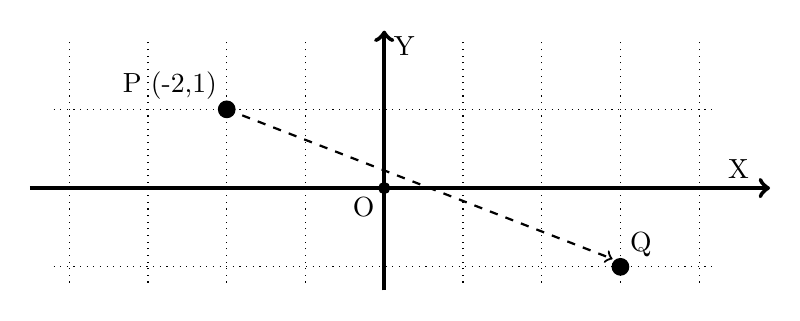
\begin{tikzpicture}
\coordinate (O) at (0,0);
\coordinate (P) at (-2,1);
\coordinate (Q) at (3,-1);
\draw [step=1cm,dotted] (-4.2,-1.2) grid (4.2,1.9);
\draw [->,ultra thick] (-4.5,0) -- (4.9,0);
\draw [->,ultra thick] (0,-1.3) -- (0,2.0);
\node [above] at (4.5,0) {X};
\node [right] at (0,1.8) {Y};
\draw [fill=black] (O) circle (2pt);
\node [below left] at (0,0) {O};
\draw [fill=black] (P) circle (3pt);
\node [above left] at (P) {P (-2,1)};
\draw [fill=black] (Q) circle (3pt);
\node [above right] at (Q) {Q};
\draw [->,thick,dashed] (P) -- (2.9,-0.9);
\end{tikzpicture}
\end{center}

\begin{cbox}[emph={complex,real,imag}]
#include <complex>
#include <cmath>
typedef complex<double> xy_t;
xy_t P(-2, 1), Q; // 初期化
cout << P << endl; // (debug用)表示
cout << P.real() << endl; // x 座標
cout << P.imag() << endl; // y 座標
Q = P + xy_t(5, -2); // 点Qは点Pを(5,-2)だけ平行移動した位置とする
Q *= xy_t(cos(a), sin(a)); // 点Qを原点を中心にa(ラジアン)だけ回転
cout << abs(P) << endl; // ベクトルOPの長さ
cout << norm(P) << endl; // \texttt{norm(P) = abs(P)}${}^2$
\end{cbox}

\paragraph{Cの複素数による表現} この資料では,Cの使用は非推奨であるが,後述する注意事項のために,一応掲載する.

C (gccまたはC99)の場合:
\begin{purecbox}[emph={complex,creal,cimag}]
#include <complex.h>
#include <math.h>
complex a = 0.0 + 1.0I; // 初期化
complex b = cos(3.14/4) + sin(3.14/4)*I;
printf("
a *= b; // 乗算
printf("
\end{purecbox}

\begin{debugbox}{乗算記号の入れ忘れに注意}
  数の\texttt{5}と変数\texttt{k}の積を求める場合は,\texttt{5*k}と書き,\texttt{5k}と書くとコンパイルエラーになる.ところが,文字\texttt{i,j,I,J}に関しては,\texttt{5j}などの表記が上記の虚数と解釈され,コンパイルエラーにはならない.\texttt{cout}に表示すると,\texttt{bool}にキャストされて\texttt{1}と表示される.知らないと見つけにくい,と思われる.
\end{debugbox}

\medskip

\paragraph{Pythonの複素数による表現} Python3においても複素数\texttt{complex}をほぼ同様に利用可能である.詳細は\texttt{help(complex)}や\texttt{help(cmath)}で確認のこと.
\begin{pybox}[emph={real,imag,complex}]
import cmath
import math
P = complex(-2,1) # \texttt{(-2+1j)}も可
print(P)
print(P.real)     # 実部
print(P.imag)     # 虚部
Q = P + complex(5,-2)     # 平行移動
Q *= complex(math.cos(a), math.sin(a))     # 回転
print(abs(P))     # 長さ
\end{pybox}
\subsection{よく使う演算}

\begin{center}
\begin{tabular}{c@{\hspace{5em}}c}
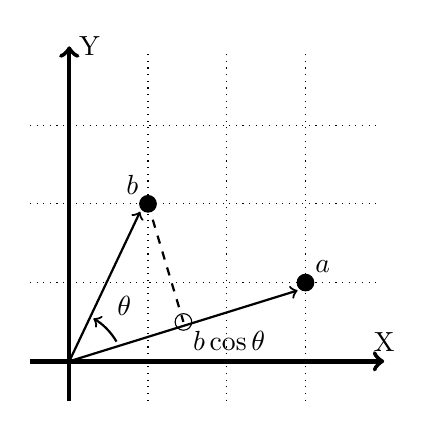
\begin{tikzpicture}
\coordinate (O) at (0,0);
\coordinate (A) at (3,1);
\coordinate (B) at (1,2);
\coordinate (BcosT) at (1.45,0.5);
\draw [step=1cm,dotted] (-0.5,-0.5) grid (3.9,3.9);
\draw [->,ultra thick] (-0.5,0) -- (4,0);
\draw [->,ultra thick] (0,-0.5) -- (0,4);
\node [above] at (4,0) {X};
\node [right] at (0,4) {Y};
\draw [fill=black] (A) circle (3pt);
\node [above right] at (A) {$a$};
\draw [fill=black] (B) circle (3pt);
\node [above left] at (B) {$b$};
\draw [] (BcosT) circle (3pt);
\node [below right] at (BcosT) {$b\cos\theta$};
\draw [->,thick] (O) -- (2.9,0.9);
\draw [->,thick] (O) -- (0.9,1.9);
\draw [->,thick] (0.6,0.25) arc (30:60:0.8);
\draw [thick,dashed] (B) -- (BcosT);
\node at (0.7,0.7) {$\theta$};
\end{tikzpicture}
&
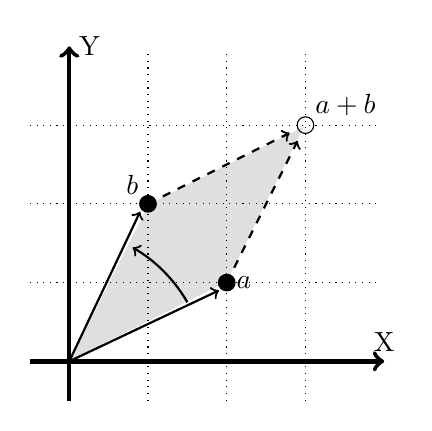
\begin{tikzpicture}
\coordinate (O) at (0,0);
\coordinate (A) at (2,1);
\coordinate (B) at (1,2);
\coordinate (AB) at (3,3);
\draw [color=white,fill=gray!25!] (O) -- (A) -- (AB) -- (B) -- cycle;
\draw [step=1cm,dotted] (-0.5,-0.5) grid (3.9,3.9);
\draw [->,ultra thick] (-0.5,0) -- (4,0);
\draw [->,ultra thick] (0,-0.5) -- (0,4);
\node [above] at (4,0) {X};
\node [right] at (0,4) {Y};
\draw [fill=black] (A) circle (3pt);
\node [right] at (A) {$a$};
\draw [fill=black] (B) circle (3pt);
\node [above left] at (B) {$b$};
\draw [] (AB) circle (3pt);
\node [above right] at (AB) {$a+b$};
\draw [->,thick] (O) -- (1.9,0.9);
\draw [->,thick] (O) -- (0.9,1.9);
\draw [->,thick] (1.5,0.75) arc (30:60:1.9);
\draw [->,thick,dashed] (A) -- (2.9,2.8);
\draw [->,thick,dashed] (B) -- (2.8,2.9);
\end{tikzpicture}
\\
(1) 内積: $|a||b|\cos\theta$ & (2) クロス(外)積: 網掛け部分の符号付き面積
\end{tabular}
\end{center}

\begin{cbox}[emph={cross_product,dot_product,projection}]
// 図(1) 内積: a.x*b.x +a.y*b.y
double dot_product(xy_t a, xy_t b) { return (conj(a)*b).real(); }
// 図(2) クロス(外)積, ベクトルa,bが作る\textcolor{ired}{三角形の符号付き面積}の二倍: a.x*b.y - b.x*a.y
double cross_product(xy_t a, xy_t b) { return (conj(a)*b).imag(); }
// (対応図なし) 投影 原点とbを結ぶ直線に点pを投影
xy_t projection(xy_t p, xy_t b) { return b*dot_product(p,b)/norm(b); }
\end{cbox}

三角形の\jindex{符号付き面積}{ふごうつきめんせき}の紹介が本章前半の主要なテーマである.これは原点と点a,bが作る三角形の面積を,符号付きで求める.符号は,原点と点a,bがこの順で反時計回りの位置関係にある場合に正,時計回りの場合に負となる.面積だけでなく,これから見るように向きの判定にも用いられる.

内積は,直線上に点を投影する際に便利である.

\begin{pybox}[emph={cross_product,dot_product,projection,norm}]
def norm(c):
    a = abs(c)
    return a*a
def dot_product(a, b):
    return (a.conjugate()*b).real
def cross_product(a,b):
    return (a.conjugate()*b).imag
def projection(p, b):
    return b*dot_product(p,b)/norm(b)  
\end{pybox}

\section{三角形の符号付き面積の利用}

\subsection{多角形の面積}
\begin{psbox}{Area of Polygon}{PC甲子園2005}
  凸多角形の面積を求めよ.

注1: 問題文中にはヘロンの公式が書いてあるが,下記の符号付き三角形で解くこと.(あとで凸でない多角形の面積に応用するため)

注2: 頂点列は順に与えられるが,時計回りか反搬時計回りかは指定がないため,最後に絶対値をとる.

\aojid{0079}
\end{psbox}

\begin{center}
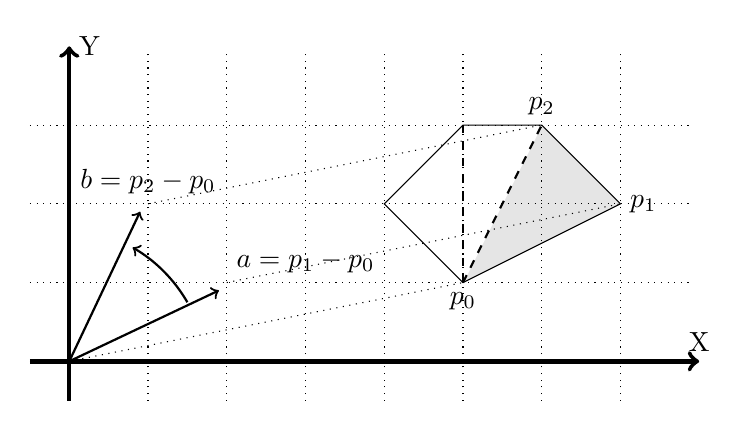
\begin{tikzpicture}
\coordinate (O) at (0,0);
\coordinate (A) at (2,1);
\coordinate (B) at (1,2);
\coordinate (P0) at (5,1);
\coordinate (P1) at (7,2);
\coordinate (P2) at (6,3);
\draw [color=white,fill=gray!20!] (P0) -- (P1) -- (P2) -- cycle;
\draw [] (P0) -- (P1) -- (P2) -- (5,3) -- (4,2) -- cycle;
\draw [step=1cm,dotted] (-0.5,-0.5) grid (7.9,3.9);
\draw [->,ultra thick] (-0.5,0) -- (8,0);
\draw [->,ultra thick] (0,-0.5) -- (0,4);
\node [above] at (8,0) {X};
\node [right] at (0,4) {Y};
\node [above right] at (A) {$a=p_1-p_0$};
\node [above] at (B) {$b=p_2-p_0$};
\draw [->,thick] (O) -- (1.9,0.9);
\draw [->,thick] (O) -- (0.9,1.9);
\draw [->,thick] (1.5,0.75) arc (30:60:1.9);
\draw [thick,dashed] (5,1) -- (6,3);
\draw [thick,dashed] (5,1) -- (5,3);
\node [below] at (P0) {$p_0$};
\node [right] at (P1) {$p_1$};
\node [above] at (P2) {$p_2$};
\draw [dotted] (A) -- (P1);
\draw [dotted] (B) -- (P2);
\draw [dotted] (O) -- (P0);
\end{tikzpicture}
\end{center}

(単純)多角形は三角形に分解できるので,三角形の面積が計算できれば,多角形の面
積が計算できる.特に凸多角形の場合は,一つの頂点とその頂点を含まない辺
が構成する三角形で綺麗に分割できる.

\begin{cbox}
xy_t P[110];
int main() {
  // 入力例 読み込んだ点の個数をNとする
  int N=0;
  double x, y;
  while (~scanf("
    P[N++] = xy_t(x,y);
  }
  // 面積計算
  double sum = 0.0;
  for (int i=0; i+2<N; ++i) {
    xy_t a=P[0], b=P[i+1], c=P[i+2];
    sum += ... // 三角形 abc の面積を加算
  }
  printf("
}
\end{cbox}

\begin{tipsbox}{scanfで入力が続く限り読む方法}
入力行を読める限り読むために,サンプルコード中では\texttt{while (\~{}scanf("\%lf,\%lf", \&x, \&y))}というループを採用した.これは,短い(しかし汎用性の低い)書き方で,\texttt{\~{}EOF}が0になる環境でのみ使用可能である.
\end{tipsbox}

\begin{pybox}
P = [] # 頂点列
try:
    while True:
        x,y = map(float,input().split(','))
        P.append(complex(x,y))
except EOFError:
    pass
N = len(P) # 頂点の個数
total = 0.0
for i in range(1,N-1):
    a,b,c = P[0],P[i],P[i+1]
    total += .. // 三角形 abc の面積を加算
print("
\end{pybox}

\begin{tipsbox}{Python3で入力が続く限り読む方法}
\texttt{input()}を試みて入力が終わっていた場合,Pythonでは\texttt{EOFError}という例外が発生するので,あらかじめ\texttt{try}で囲み\texttt{except}で検知する.例外が発生すると\texttt{input()}の書かれていた\texttt{while}ループを脱出して,外側の\texttt{except}ブロックが実行される(この場合は\texttt{pass}で,何もせずに次の行に移る).
\end{tipsbox}

\begin{psbox}{Polygon - Area}{AOJ}
多角形の面積を計算する.凸とは限らないが,頂点は反時計回りで与えられる.  

\aojid{CGL_3_A}

(類題: Area of Polygons (国内予選1998) \aojid{1100} 頂点が与えられる向きのみ異なる)
\end{psbox}
凸でない単純多角形に対して,先ほどと同様の分割を行うと三角形に重なりが生ずるが,ここで符号付き面積の符号も含めて合計すると,(不思議なことに)正しい面積を得られる.多角形の頂点は反時計回りに順に与えられている必要がある.なお分割の中心として$p_0$を使ったが,任意の点(たとえば原点)と各辺の作る三角形を考えても良い.

\begin{center}
  \begin{tabular}{ccc}
\begin{tikzpicture}[scale=0.8]
\coordinate (P0) at (2.5,1.5);
\coordinate (P1) at (5,1);
\coordinate (P2) at (3,3);
\coordinate (P3) at (6,3);
\coordinate (P4) at (2,4);
\draw [color=iblue,fill=gray!20!,thick,dashed] (P0) -- (P1) -- (P2) -- cycle;
\draw [] (P0) -- (P1) -- (P2) -- (P3) -- (P4) -- cycle;
\node [below] at (P0) {$p_0$};
\node [right] at (P1) {$p_1$};
\node [above] at (P2) {$p_2$};
\node [right] at (P3) {$p_3$};
\node [left] at (P4) {$p_4$};
\draw [->,ultra thick,dotted,color=iblue] ($(P0)+(1.0,0.6)$) ++(-60:0.5) arc (-60:210:0.5);
1\end{tikzpicture}
&
\begin{tikzpicture}[scale=0.8]
\coordinate (P0) at (2.5,1.5);
\coordinate (P1) at (5,1);
\coordinate (P2) at (3,3);
\coordinate (P3) at (6,3);
\coordinate (P4) at (2,4);
\draw [color=iblue,fill=gray!20!,thick,dashed] (P0) -- (P2) -- (P3) -- cycle;
\draw [] (P0) -- (P1) -- (P2) -- (P3) -- (P4) -- cycle;
\node [below] at (P0) {$p_0$};
\node [right] at (P1) {$p_1$};
\node [above] at (P2) {$p_2$};
\node [right] at (P3) {$p_3$};
\node [left] at (P4) {$p_4$};
\draw [->,ultra thick,dotted,color=ired] ($(P0)+(1.6,0.7)$) ++(235:0.5) arc (235:-30:0.5);
\end{tikzpicture}
&
\begin{tikzpicture}[scale=0.8]
\coordinate (P0) at (2.5,1.5);
\coordinate (P1) at (5,1);
\coordinate (P2) at (3,3);
\coordinate (P3) at (6,3);
\coordinate (P4) at (2,4);
\draw [color=iblue,fill=gray!20!,thick,dashed] (P0) -- (P3) -- (P4) -- cycle;
\draw [] (P0) -- (P1) -- (P2) -- (P3) -- (P4) -- cycle;
\node [below] at (P0) {$p_0$};
\node [right] at (P1) {$p_1$};
\node [right] at (P3) {$p_3$};
\node [left] at (P4) {$p_4$};
\draw [->,ultra thick,dotted,color=iblue] ($(P0)+(0.6,1.3)$) ++(-60:0.5) arc (-60:210:0.5);
\end{tikzpicture}
\\
$p_0p_1p_2$ (sgn: +)
&
$p_0p_2p_3$ (sgn: -)
&
$p_0p_3p_4$ (sgn: +)
  \end{tabular}
\end{center}


  
\subsection{平行の判定}

\begin{psbox}{Parallelism}{PC甲子園2003}
概要: A = (x1, y1), B = (x2, y2), C = (x3, y3), D = (x4, y4) の異なる4つの座標点が与えられたとき,直線 AB と CD が平行かどうかを判定せよ.

点の座標は小数点以下最大 5 桁までの数字を含む実数で与えられる(この情報を数値誤差の推定に用いる).

\aojid{0021}
\end{psbox}

回答方針: ベクトルABとベクトルCDからなる三角形が面積を持つかどうかを判定すれば良い

\begin{cbox}[emph={eps}]
const double eps = 1e-11;
double x[4], y[4];
int N;
int main() {
    cin >> N; // 問題数
    for (int t=0; t<N; ++t) {
        for (int i=0; i<4; ++i) 
            cin >> x[i] >> y[i]; // x0,y0..x3,y3
        xy_t a[2] = {
            xy_t(x[0],y[0]) - xy_t(x[1],y[1]), 
            xy_t(x[2],y[2]) - xy_t(x[3],y[3])
        };
        bool p = abs(a[0]とa[1]の符号付き面積) < eps;
        cout << (p ? "YES" : "NO") << endl;
    }
}
\end{cbox}

補足: 向きや角度の判定には,\texttt{sin}や\texttt{arg}などのライブラリ
関数を用いることもできるが,計算誤差の観点から可能な限り符号付き面積で
計算するほうが良い.たとえば三角関数の汎用的な実装方法ではTaylor展開が用いられる.
\footnote{参考: FreeBSDの実装 \url{https://svnweb.freebsd.org/base/release/10.1.0/lib/msun/src/k_cos.c?view=markup}}

\begin{pybox}
N = int(input())
for _ in range(N):
    P = list(map(float,input().split()))
    a, b, c, d = [complex(P[i*2],P[i*2+1]) for i in range(4)]
    parallel = ... # abとcdが並行かを表す真偽値を計算
    print("YES" if parallel else "NO")
\end{pybox}

\begin{debugbox}{動作確認}
  この問題はサンプル入出力例が少なく,またジャッジデータも非公開である.そのため,自分でテストデータを試すと良い.たとえば,長い線,短い線,面積の符号の正負などが,確認すべき例である.

たとえば,以下の例は全て ``NO''である.
  \begin{terminal}
-0.00001 0 0.00001 0 -0.0001 0 0.00001 0.00001
-100 100 100 100 -100 100 100 99.99999
  \end{terminal}
\end{debugbox}

\medskip

\paragraph{数値誤差の取り扱い$\star$}
\texttt{double}などの浮動小数を用いる時には,$\frac{1}{2}$の冪乗の和で
表される数値以外は,必然的に誤差を含む(\ref{section:floating-point-numbers}章も参照).この問題での入力は,絶対値が100以下かつ各値
は小数点以下最大5桁までの数値と明示されているの
で,$10^5$倍して整数(\texttt{long long})で扱えば誤差の影響を避けることができる.
あるいは,サンプルコードの\texttt{eps}のように,誤差の範囲を予測する方法もある.
二つのベクトル$(a,b)$と$(c,d)$にそれぞれの要素に誤差が加わった時に,
(1)平行の場合に$|ad-bc|$の取る最大値(誤差がなければ$0$)と,(2)平行でない場合に$|ad-bc|$の取る最小値を比較して,(1)$<$閾値$<$(2)となるよう閾値をとる.
粗く見積もると(1)は最大
$(4\cdot100)\cdot(100\cdot2^{-54})\approx2.2\cdot10^{-12}$程度
($100\cdot2^{-54}$は100までの数を\texttt{double}で表した時の表現誤差,400は
$|(a+\varepsilon)(d+\varepsilon)-(b+\varepsilon)(c+\varepsilon)|$を展開した時の
$\varepsilon$にかかる係数の見積もり), 
(2)は$10^{-10}$程度(入力が表現可能な$10^{-5}$値の自乗より).
なお,環境依存になるが比較的新しいIntelやAMDのCPUと比較的新しいgccを用いる場合は,\texttt{long double}や
\texttt{\_\_float128} などを用いることで80~bit や128~bitというより良い精度で演算することもできる.それぞれ注意点があるので,使用する場合は文献を調査のこと.

\subsection{内外判定}

\begin{psbox}{A Point in a Triangle}{PC甲子園2003}
平面上に (x1, y1), (x2, y2), (x3, y3) を頂点とした三角形と点 P(xp, yp) がある.点 P が三角形の内部(三角形の頂点や辺上は含まない)にあるかどうかを判定せよ.

\aojid{0012}
\end{psbox}
    
回答例: 三角形の各点をa,b,cとすると,3つの三角形 pab, pbc, pca の符号付き面積を考える.pがabcの内部にあれば符号は一致し,外部にあれば一致しない.

\begin{tabular}{c@{\hspace{3em}}c}
\begin{tikzpicture}[x=2mm,y=2mm]
\fill[ired] (10,10) circle (0.5);
\node[above right] at (10,10) {$p$};
\node[right] at (20,0) {$a$};
\node[above] at (10,20) {$b$};
\node[left] at (0,5) {$c$};
\draw[->, thick] (20,0) edge node [left] {\small 左} (10,20);
\draw[->, thick] (10,20) edge node [right] {\small 左} (0,5);
\draw[->, thick] (0,5) edge node [above] {\small 左} (20,0);
\draw[dotted] (20,0) -- (10,10);
\draw[dotted] (10,20) -- (10,10);
\draw[dotted] (0,5) -- (10,10);
  \begin{scope}[xshift=57,yshift=57,rotate=20]
\draw [->,ultra thick,dotted,color=iblue] (0,0) ++(-30:2.5) arc (-30:90:2.5);
\draw [->,ultra thick,dotted,color=iblue] (0,0) ++(90:2.5) arc (90:210:2.5);
\draw [->,ultra thick,dotted,color=iblue] (0,0) ++(210:2.5) arc (210:330:2.5);
  \end{scope}
\end{tikzpicture}
&
\begin{tikzpicture}[x=2mm,y=2mm]
\fill[ired] (18,15) circle (0.5);
\node[above right] at (18,15) {$p$};
\node[right] at (20,0) {$a$};
\node[above] at (10,20) {$b$};
\node[left] at (0,5) {$c$};
\draw[->] (20,0) edge node [right] {\small 右} (10,20);
\draw[->] (10,20) edge node [right] {\small 左} (0,5);
\draw[->] (0,5) edge node [above] {\small 左} (20,0);
\draw[dotted] (20,0) -- (18,15);
\draw[dotted] (10,20)-- (18,15);
\draw[dotted] (0,5)  -- (18,15);
  \begin{scope}[xshift=57,yshift=57,rotate=20]
\draw [->,ultra thick,dotted,color=ired] (0,0) ++(90:2.5) arc (90:-30:2.5);
\draw [->,ultra thick,dotted,color=iblue] (0,0) ++(90:2.5) arc (90:210:2.5);
\draw [->,ultra thick,dotted,color=iblue] (0,0) ++(210:2.5) arc (210:330:2.5);
  \end{scope}
\end{tikzpicture}\\
点が図形の内部 & 点が図形の外部
\end{tabular}

\begin{cbox}
double x[4], y[4];
int main() {
    while (true) {
        for (int i=0; i<4; ++i) cin >> x[i] >> y[i];
        if (!cin) break;
        xy_t a(x[0],y[0]), b(x[1],y[1]), c(x[2],y[2]), p(x[3],y[3]);
        // pab の符号付き面積の2倍は,\texttt{cross\_product(a-p,b-p)}
        // pbc の符号付き面積の2倍は,\texttt{cross\_product(b-p,c-p)}
        // pca の符号付き面積の2倍は,\texttt{cross\_product(c-p,a-p)}
        bool ok = 符号が揃っている
        cout << (ok ? "YES" : "NO") << endl;
    }
}
\end{cbox}

凸とは限らない多角形の内外判定については,次の節を参照.

\subsection{凸包}

\begin{pbox}{Convex Polygon - Convex Hull$\star$}{AOJ}
与えられた点の集合の凸包を求めよ.凸包が何かは類題の図を参照.

(注: 辺上の点を出力させる,少し特殊な設定である)

\aojid{CGL_4_A}

(類題: Enclose Pins with a Rubber Band (PC甲子園2004) \aojid{0068} こちらの方が素直な設定)
\end{pbox}

回答例: 点をX座標でソートし,最小値(左端の点)から順に右に向かい,まずは下半分の外周を構成する.
途中現在の進行方向より右に向かうことになったら,(本来凸法に含まれない点
を入れてしまった状況であるので)原因となった点をすべて取り除く.上半分も
右端から同様に行う.

点の個数を$N$とすると,上記の半周を求める手続きは$O(N)$でできるため,ソートに要する時間を含めて全体の計算時間は$O(N\log N)$.

\begin{center}
\begin{tabular}{c@{\hspace{3em}}c@{\hspace{3em}}c}
\begin{tikzpicture}[scale=0.8]
\coordinate (P0) at (2,4);
\coordinate (P1) at (2.5,1.5);
\coordinate (P2) at (3,3);
\coordinate (P3) at (5,1);
\coordinate (P4) at (6,3);
\draw [] (P0) circle (2.5pt);
\draw [] (P1) circle (2.5pt);
\draw [] (P2) circle (2.5pt);
\draw [] (P3) circle (2.5pt);
\draw [] (P4) circle (2.5pt);
\draw (P0) -- (P1);
\end{tikzpicture}
&
\begin{tikzpicture}[scale=0.8]
\coordinate (P0) at (2,4);
\coordinate (P1) at (2.5,1.5);
\coordinate (P2) at (3,3);
\coordinate (P3) at (5,1);
\coordinate (P4) at (6,3);
\draw [] (P0) circle (2.5pt);
\draw [] (P1) circle (2.5pt);
\draw [] (P2) circle (2.5pt);
\draw [] (P3) circle (2.5pt);
\draw [] (P4) circle (2.5pt);
\draw (P0) -- (P1) -- (P2);
\end{tikzpicture}
&
\begin{tikzpicture}[scale=0.8]
\coordinate (P0) at (2,4);
\coordinate (P1) at (2.5,1.5);
\coordinate (P2) at (3,3);
\coordinate (P3) at (5,1);
\coordinate (P4) at (6,3);
\draw [] (P0) circle (2.5pt);
\draw [] (P1) circle (2.5pt);
\draw [] (P2) circle (2.5pt);
\draw [] (P3) circle (2.5pt);
\draw [] (P4) circle (2.5pt);
\draw (P0) -- (P1) -- (P2);
\draw[thick,dashed] (P2) -- (P3);
\end{tikzpicture}
\\
t=0: 左端(x座標最小)から
&
t=1: 順に線をつなぐ
&
t=2: 右向きになったら
\\
\begin{tikzpicture}[scale=0.8]
\coordinate (P0) at (2,4);
\coordinate (P1) at (2.5,1.5);
\coordinate (P2) at (3,3);
\coordinate (P3) at (5,1);
\coordinate (P4) at (6,3);
\draw [] (P0) circle (2.5pt);
\draw [] (P1) circle (2.5pt);
\draw [] (P2) circle (2.5pt);
\draw [] (P3) circle (2.5pt);
\draw [] (P4) circle (2.5pt);
\draw (P0) -- (P1) -- (P3);
\end{tikzpicture}
&
\begin{tikzpicture}[scale=0.8]
\coordinate (P0) at (2,4);
\coordinate (P1) at (2.5,1.5);
\coordinate (P2) at (3,3);
\coordinate (P3) at (5,1);
\coordinate (P4) at (6,3);
\draw [] (P0) circle (2.5pt);
\draw [] (P1) circle (2.5pt);
\draw [] (P2) circle (2.5pt);
\draw [] (P3) circle (2.5pt);
\draw [] (P4) circle (2.5pt);
\draw (P0) -- (P1) -- (P3) -- (P4);
\end{tikzpicture}
\\
t=4: 必要なだけ点を削除してつなげ直し
&
t=5: 下側完成
\end{tabular}
\end{center}

\paragraph{点の整列}

C++の複素数型(complex)には,比較演算子が定義されていないので,自分で定義する必要がある.下記の例のように\texttt{std}ネームスペースで\texttt{operator<}を定義すると,\texttt{sort}で自動で使われる.
比較基準としては,\texttt{!(a<b)}かつ\texttt{!(b<a)}の場合に\texttt{a==b}であるようなものを用いること.\footnote{\url{https://en.cppreference.com/w/cpp/named_req/Compare}}

\begin{cbox}[emph={std}]
namespace std {
  bool operator<(xy_t l, xy_t r) {
    return (l.real()!=r.real()) ? l.real()<r.real() : l.imag())<r.imag();
  }
  // 別案: std::pairと揃える場合
  bool operator<(xy_t l, xy_t r) {
    return make_pair(l.real(), l.imag()) < make_pair(r.real(), r.imag());
  }
}
  
\end{cbox}

\section{様々な話題}

\begin{psbox}{A Symmetric Point}{PC甲子園2005}
点Qと線対称の位置にある点を出力せよ.

\aojid{0081}
\end{psbox}

回答例: 直線上にQを投影した点をSとする.すると求める点Rは,SをベクトルQSだけ平行移動した位置にある.カンマ区切りで与えられる入力の処理と,また小数点以下の出力桁数の制御には,\texttt{\#include<cstdio>}して以下のように\texttt{scanf}と\texttt{printf}を用いるのが簡便である.

\begin{cbox}
#include <cstdio>
double X1,Y1,X2,Y2,XQ,YQ;
  
int main() {
  while (~scanf("
                 &X1, &Y1, &X2, &Y2, &XQ, &YQ)) {
    xy_t P1(X1,Y1), P2(X2,Y2), Q(XQ,YQ);
    xy_t R = ...; // 線対称の点を計算
    printf("
  }
}
\end{cbox}

\begin{pbox}{Polygon - Polygon-Point Containment}{AOJ}
凸とは限らない多角形について点の内外を判定せよ.

\aojid{CGL_3_C}
\end{pbox}
(注: 通常は点が辺上かどうかを判定することは難しいが,今回は整数座標なので可能)

回答例: 調べたい点から任意の方向に半直線を伸ばし,横切る辺の数を数える.偶数ならば外部,奇数ならば内部である.線分が直線と交点を持つかどうかなどの関数を事前に用意しておく必要がある.半直線が頂点のすぐ近くを通過する場合は,誤差の影響を心配しないで済むよう,角度を変えたほうが無難.

\begin{pbox}{Point Set - Closest Pair$\star$}{AOJ}
最近点対を求めよ.  

\aojid{CGL_5_A}
\end{pbox}

点の個数を$N$して,点のペアを全て試すと$O(N^2)$の時間が必要だが,分割統
治により$O(N\log N)$で可能.なお$O(N)$の乱択アルゴリズムも存在する.

分割統治の方針: X座標毎とY座標毎のそれぞれで点をソートしておく.X座標で点を半分に分
け,左と右でそれぞれ最近点対を再帰的に求める.求めた二つの最小距離の小さい方を$d$とする.全体
の最近点対は,左のみの最近点対,右のみの最近点対,左の点と右の点の最近
点対のいずれかである.後者は左右の区切りの線から距離$d$以内のものについ
てY座標順に並べた時に,定数(たとえば8)以内のペアのみ候補となる性質を用いると,点
の個数に対して線形の計算ステップで判定可能である.証明は区切りの線の周囲の適
当な正方形グリッドを考えると,$d$の制限で点があまり密に存在できないこと
から.なお,実装では,毎回Y座標順にソートしていると$O(N\log N)$を実現で
きない.初めに一度全体をソートしておき,分割の際にそこから振り分けると良
い.また分割の際には,複数の点が同じY座標を持つ場合に注意を払う必要があ
りうる.実用的には,初めに全体をランダムに回転させると避けられる.

\section{応用問題}

\begin{pbox}{ConvexCut}{夏合宿2012}
与えられた図形に,どの角度で分割しても同じ面積で切れるような点が存在するかを求める.

\aojid{2442}
\end{pbox}

多角形の頂点が偶数であり,かつ組みになるべき辺が全て平行である時に限ら
れること,あるいは組になる頂点の中点が等しいことなどで判定できることが
証明できる.

回答例(入出力)
\begin{cbox}
#include <complex>
#include <iostream>
#include <cstdio>
using namespace std;
int N, x, y;
typedef complex<double> xy_t;
xy_t P[60];
void solve() {
 ...
}
int main() {
    while (cin >> N) {
        for (int i=0; i<N; ++i) {
            cin >> x >> y;
            P[i] = xy_t(x,y);
        }
        solve();
    }
} 
\end{cbox}

回答例(中点の計算)
\begin{cbox}
void solve() {
  // 奇数だったらそのような点はない
  ...
  xy_t a = (P[0]+P[N/2])*0.5; // P[0]とP[N/2]の中点
  for (int i=1; i<N/2; ++i) {
    xy_t b = ... // P[i]とP[i+N/2]の中点
    // aとbが誤差を加味しても一致していなければ,abs(a-b) > eps,求める点はない
  }
  printf("
}  
\end{cbox}

\begin{pbox}{Circle and Points$\star$}{国内予選2004}
xy平面上にN個の点が与えられる.半径1の円をxy平面 上で動かして,それらの点をなるべくたくさん囲むようにする.このとき,最大でいくつの点を同時に囲めるかを答えなさい.ここで,ある円が点を「囲む」 とは,その点が円の内部または円周上にあるときをいう. (この問題文には誤差に関する十分な記述がある)

\aojid{1132}
\end{pbox}

候補となる円の位置は無数にあるので,候補を絞る.
(「ぎりぎりを考えよ」\pccbook[p.~229])

\begin{tipsbox}{考え方}
同時に囲める最大の点をnとして,n個を囲んだ円があったとする.もしその円
に点が接してないのであれば,内部の点のどれかが接するまで動かしても,囲
んでいる点の数は変わらない.
すなわち,点のどれかと接する円だけを考えれば十分である(残りの円を考慮に入れても,答えは変わらない).しかしそのような円はまだ無数にある.

n個を囲んだ円があり,一点が円上に乗っているとする.その点を\textcolor{white}{中心に円を回転させると,内部の点が新たに円と接するまで動かしても,囲んでいる点の数はかわらない.
すなわち,2点を通る円だけを考えれば十分である(残りの円を考慮に入れても,答えは変わらない).そのような円は$2N^2$程度の個数}しかない.
\end{tipsbox}

\begin{debugbox}{例外ケースに注意}
上記の考え方は概ね正しいが,例外ケースがある.すなわち答えが\textcolor{white}{1の時は,最大を与える円は}上記の性質を持たない.
\end{debugbox}

\begin{debugbox}{点の数え方}
  ある点pにピッタリ載る円の位置を設定し,それに含まれる点の個数を調べたいとする.そのためには全ての点について円の中心との距離を計算すれば,概ね判定可能である.しかし,点pそのものについては,円上に位置するため,数値誤差により外と判定されてしまうかもしれない.ここで許容誤差を大きくすると,本当に外にある点を内と判定してしまうリスクがある.そのため点pの判定は特別扱いし,\textcolor{white}{距離を計算せずに,id (点を配列で管理しているなら何番目か)の同一性を用いると良い.}
\end{debugbox}

回答例:

\begin{cbox}
int main() {
  // 最大値を初期化
  for (/*点p*/) {
    for (/*点q*/) { // p!=q
      if (/*pqを通る円があれば*/) { // 0個,1個,2個の場合がある
         /*全ての点を確かめながら,内部の個数を数える*/
         /*最大値を越えていれば更新する*/
      }
    }
  }
}
\end{cbox}


\begin{pbox}{Roll-A-Big-Ball}{国内予選2008}
条件を満たす最大の大玉の大きさを求める.

  \aojid{1157}
\end{pbox}

\begin{pbox}{Space Golf}{アジア大会2014}
  
  \aojid{1348}
\end{pbox}

\begin{pbox}{Chain-Confined Path$\star$}{国内予選2012}
  円環を通る最短経路を求めよ.

\aojid{1183}
\end{pbox}

ヒント: 最短経路の形状を考える
 
解法: \textcolor{white}{始点,終点,各円の交点を頂点とし,各点の間を直線で移動可能かを求めて辺を張り,最短路問題を解く.}

\begin{pbox}{Neko's Treasure$\star$}{模擬地区予選2009}
壁をいくつ乗り越えるかを求める(問題文参照)

\aojid{2181}
\end{pbox}

\begin{pbox}{Area of Polygons$\star$}{アジア大会2003}
網掛け部分の面積を求める.

\aojid{1242}
\end{pbox}
考え方: 薄切りにして和を求めるだけなのだが,複数の線が同じますを通る場合など,注意点がそれなりにある.

参考: \url{http://www.ipsj.or.jp/07editj/promenade/4501.pdf}

\begin{pbox}{Treasure Hunt$\star$}{夏合宿2012}
領域内の宝を(効率的に)数える

\aojid{2426}
\end{pbox}

純朴に数えていると時間がかかりすぎるので,点が与えられた時点で前処理を
行い,質問に答える準備を整えておく.
質問に効率的に答えるためのデータ構造としては,たとえば四分木(\textbf{quad tree})を使うことができる.



\begin{pbox}{Altars$\star\star$}{6th Polish Olympiad in Informatics}
中国では悪霊は直線上に進むと信じられているという枕.

長方形の寺院があり,中央に祭壇がある.寺院の壁は,東西または南北のいずれかの方向からなる.寺院の入り口は,ある辺の中央にある.外部から祭壇に視線が通っているかどうかを調べよ.

\url{http://main.edu.pl/en/archive/oi/6/olt}  
\end{pbox}

\begin{pbox}{Fish$\star\star$}{Algorithmic Engagements 2009}
毎日同じ時刻に起床/就寝する魚がいる.寝て起きると,海流の影響で一マスずれていることがある.昨日の同時刻の自分の位置が見えるように泳ぐ.加減速は自在.一日の魚の動きを観察したルートの記録がたくさんあるが,日付が分からない.最小で何尾の魚を観察していると言えるか.

archipelago=群島

\url{http://main.edu.pl/en/archive/pa/2009/ryb}  
\end{pbox}
 \chapter{簡単な構文解析}\label{chapter:parsing}

\begin{itembox}[l]{こんな問題}
特定の文法で書かれた文字列を計算機に理解させよう:
  \begin{itemize}
\setlength{\itemsep}{0pt}
  \item $( V | V ) \& F \& ( F| V)$ \dingright $F$ (真偽値の計算)
  \item 35=1?((2*(3*4))+(5+6)) \dingright '+'  (演算子の推定)
  \item 4*x+2=19 \dingright x=4.25 (方程式を解く)
  \item C2H5OH+3O2+3(SiO2) == 2CO2+3H2O+3SiO2 (分子量の計算)
  \end{itemize}  
\end{itembox}

\section{四則演算の作成}

\subsection{足し算を作ってみよう}

\paragraph{大域変数}:
\begin{cbox}
const string S = "12+3";
size_t cur = 0; // 解析開始位置 cursorの略記
int parse();
\end{cbox}

実行例: (以下のように動作するものをこれから作る)
\begin{cbox}
int main() {
  int a = parse();
  assert(a == 15);
  assert(cur == S.size());
}  
\end{cbox}

\begin{pybox}
S = "0"
cur = 0

a = parse()
assert a == 15
assert cur == len(S)
\end{pybox}

\paragraph{1文字読む関数の準備}

\begin{cbox}[emph={readchar,peek}]
// 1文字読んでcurを進める
char readchar() { 
  assert(cur < S.size());    
  char ret = S[cur];
  cur += 1;
  return ret;
  // return S[cur++]; と一行で書くこともできる
}
// 1文字読むがcurを進めない
char peek() { 
  assert(cur < S.size());    
  return S[cur];
}
\end{cbox}

Pythonで,関数内でグローバル変数を変更するには,\tindex{global}で指定する.
\begin{pybox}[emph=global]
def readchar():
    global cur
    c = S[cur]
    cur += 1
    return c
def peek():
    return S[cur]
\end{pybox}

\paragraph{assertって何?} 
(再掲)
\begin{cbox}[emph={cassert,assert}]
#include <cassert>
int factorial(int n) {
  assert(n > 0); // (*)
  if (n == 1) return 1;
  return n * factorial(n-1);
}     
\end{cbox}

実行例
\begin{cbox}
cout << factorial(3) << endl; // 6を表示
cout << factorial(-3) << endl; // (*)の行番号を表示して停止
\end{cbox}

\subsubsection{最初の足し算}

\begin{itembox}[l]{足し算の(いい加減な)文法}
  \begin{alltt}
Expression := Number '+' Number
Number := Digitの繰り返し
Digit := '0' | '1' | ... | '9'\end{alltt}  
\end{itembox}

読みかた: (参考: (Extended) BNF)
\begin{itemize}
\setlength{\itemsep}{0pt}
\item \texttt{P := Q} \dingright Pという名前の文法規則の定義
\item \texttt{A B} \dingright Aの後にBが続く
\item \texttt{'a'} \dingright 文字a
\item \texttt{x | y} \dingright xまたはy
\end{itemize}


\subsubsection{文法通りに実装する (Digit)}
\texttt{\textcolor{ired}{Digit := '0' | '1' | ... | '9'}}

\begin{cbox}[emph={digit,peek,readchar}]
#include <cctype>
int digit() {
  assert(isdigit(peek()));  // S[cur]が数字であることを確認
  int n = readchar() - '0'; // '0'を0に変換
  return n;
}
\end{cbox}
文字の数字への変換: CやC++では文
字はその文字を表す数字で管理される.言語の規格では文字コードが規定されていないが,
現状で我々が使う環境では\eindex{ASCII}コードと考えて良い.その中
で,'0','1','2',$\ldots$,'a','b','c'などの文字の順番でコードが割り当て
られていることを利用すると,上記の減算により'0'からいくつ後の文字かが
分かり,それがすなわち求めたい数値である.ASCIIコード表を確認する手段の一つは,manコマンドが簡便で,ターミナルで\texttt{man ascii}とすると良い.

\begin{pybox}
def digit():
  assert peek().isdigit()
  n = int(readchar()) # 1文字読んで数値に変換
  return n;
\end{pybox}

Pythonの場合は,上記のように\texttt{isdigit()}で判定し,\texttt{int}で変換すると良い.

\subsubsection{文法通りに実装する (Number)}
\texttt{\textcolor{ired}{Number := Digitの繰り返し}}

\begin{cbox}[emph={number},emph={[2]digit}]
int number() {
  int n = digit();
  while (cur < S.size() && isdigit(peek())) // 次も数字か1文字先読
    n = n*10 + digit(); 
  return n;
}
\end{cbox}

\begin{pybox}[emph={number},emph={[2]digit}]
def number():
    n = digit()
    while cur < len(S) and peek().isdigit():
        n = n*10+digit()
    return n  
\end{pybox}

\subsubsection{文法通りに実装する (Expression)}
\texttt{\textcolor{ired}{Expression := Number '+' Number}}

\begin{cbox}[emph={expression},emph={[2]number}]
int expression() {
  int a = number();
  char op = readchar();
  int b = number();
  assert(op == '+');
  return a + b;
}
\end{cbox}

足し算だけならこれで動くはずである:
\begin{cbox}
const string S = "12+3";
size_t cur = 0; // 解析開始位置
.. 
int parse() { return expression(); }
int main() {
  int a = parse();
  cout << a << endl; // 15が出力されるはず;
}  
\end{cbox}

\paragraph{テスト}
``12+5''以外にも ``1023+888''など試してみよう

\subsubsection{拡張: 引き算を加えよう}
``12+5''を ``12-5''としてみよう

方法: expression関数でopが'+'か'-'を判定する
\begin{cbox}
  if (op == '+') return a + b;
  else return a - b;  
\end{cbox}
(assertも適切に書き換える)

\subsubsection{拡張: 3つ以上足す}
``12+5''を ``1+2+3+4''としてみよう

expressionを書き換えて,複数回足せるようにする
\begin{cbox}[emph={sum,while}]
int expression() {
    int sum = number();
    while (cur < S.size() && (peek() == '+' || peek() == '-')) {
        // 足し算か引き算が続く間
        char op = readchar();
        int b = number();
        if (op == '+') sum にbをたす;
        else sum からbを引く;
    }
    return sum;
}
\end{cbox}


\subsubsection{次の拡張}
  \begin{itemize}
\setlength{\itemsep}{0pt}
  \item 掛け算,割り算に対応: \\
    演算子の優先順位が変わるので新しい規則を作る
  \item (多重の)カッコに対応: \\
    同新しい規則を作って再帰する
  \end{itemize}

\subsection{カッコを使わない四則演算の(いい加減な)文法}

\begin{itembox}[l]{四則演算の(いい加減な)文法}
  \begin{alltt}
Expression := Term \{ ('+'|'-') Term \}
Term := Number \{ ('*'|'/') Number \}
Number := Digit \{ Digit \}
\end{alltt}
\end{itembox}

読みかた: (参考: (Extended) BNF)
\begin{itemize}
\setlength{\itemsep}{0pt}
\item \texttt{A B} \dingright Aの後にBが続く
\item \texttt{\{C\}} \dingright Cの0回以上の繰り返し
\end{itemize}

例: 5*3-8/4-9
\begin{itemize}
\setlength{\itemsep}{0pt}
\item Term: 5*3, 8/4, 9
\item Number: 5, 3, 8, 4, 9
\end{itemize}

\subsubsection{四則演算の実装 (Term)}
\texttt{\textcolor{ired}{Term := Number \{ ('*'|'/') Number \}}}

  \begin{cbox}[emph={term},emph={[2]number,*,/}]
int term() {
  int a = number();
  while (cur < S.size() 
        && (peek() == '*' || peek() == '/')) {
    char op = readchar();
    int b = number();
    if (op == '*') a *= b; else a /= b;
  }
  return a;
}
\end{cbox}

Pythonでは,\texttt{//}演算子で整数除算が可能だが,この問題の仕様とは少し異なる.すなわち,この問題では\texttt{3/-2}を-2ではなく-1と評価する必要があるようである.そこで,\texttt{math.}\tindex{trunc}関数を用いる.
\begin{pybox}[emph={term},emph={[2]number,*,/}]
import math
def term():
    a = number()
    while cur < len(S) and (peek() == '*' or peek() == '/'):
        op = readchar()
        b = number()
        a = a*b if op == '*' else math.trunc(a/b)
    return a
\end{pybox}
  
\subsubsection{四則演算の実装 (Expression)}
\texttt{\textcolor{ired}{Expression := Term \{ ('+'|'-') Term \}}}

  \begin{cbox}[emph={expression},emph={[2]term,+,-}]
int expression() {
  int a = term();
  while (cur < S.size())
      && (peek() == '+' || peek() == '-')) {
    char op = readchar();
    int b = term();
    if (op == '+') a += b; else a -= b;
  }
  return a;
}
\end{cbox}

\subsection{四則演算: カッコの導入}
式全体を表すExpressionが,カッコの中にもう一度登場 \dingright 再帰的に
処理

\begin{itembox}[l]{カッコを導入した文法}
  \begin{alltt}
Expression := Term \{ ('+'|'-') Term \}
Term := \textcolor{ired}{Factor} \{ ('*'|'/') \textcolor{red}{Factor} \}
\textcolor{ired}{Factor := '(' Expression ')' | Number}
\end{alltt}
\end{itembox}

\texttt{factor()}の実装例は以下:
  \begin{cbox}[emph={factor},emph={[2]number,expression}]
int expression(); // 前方宣言
int factor() {
  if (peek() != '(') return number();
  readchar(); // '('を読み捨てる
  int n = expression();
  assert(peek() == ')');
  readchar(); // ')'を読み捨てる
  return n;
}
\end{cbox}

\texttt{term()}の実装も,文法に合わせて調整すること.

\subsection{まとめ}
実装のまとめ:
  \begin{itemize}
\setlength{\itemsep}{0pt}
  \item 文法規則に対応した関数を作る
  \item 帰り値の型は解析完了後に欲しいものとする
    \begin{itemize}
\setlength{\itemsep}{0pt}
    \item 四則演算 \dingright 整数
    \item 多項式 \dingright 各次数の係数
    \item 分子式 \dingright 分子量,各原子の個数…
    \end{itemize}
  \end{itemize}

文法の記述:
  \begin{itemize}
\setlength{\itemsep}{0pt}
  \item 注意点: 演算子の優先順位や左結合や右結合
  \item 制限: 1文字の先読みで適切な規則を決定できるように (LL(1))
  \end{itemize}


\paragraph{補足}

\texttt{P := A \{ '+' A \}} の繰り返しを再帰で記述する?
\begin{itemize}
\setlength{\itemsep}{0pt}
\item \texttt{P := P '+' A | A}\\
\dingright このまま実装するとPでずっと再帰
\item 右結合に変換すると一応解析可能
  \begin{itemize}
\setlength{\itemsep}{0pt}
  \item \texttt{P := A P'}
  \item \texttt{P' := '+' A P' | $\epsilon$}
  \end{itemize}
($\epsilon$は空文字列)
\end{itemize}

\section{練習問題}

\begin{pbox}{Smart Calculator}{PC甲子園2005}
電卓を作る

  \aojid{0109}
\end{pbox}

回答例:
\begin{cbox}
/*const*/ string S; // 値を変更するのでconst属性を削除
...
int main() {
    int N;
    cin >> N;
    for (int i=0; i<N; ++i) {
        cur = 0;
        cin >> S;
        S.resize(S.size()-1); // 最後の=を無視
        cout << expression() << endl;
    }
}  
\end{cbox}

\begin{pbox}{Molecular Formula}{アジア地区予選2003}
各原子の原子量を元に,各分子の分子量を求める.

\aojid{1244}
\end{pbox}

初めに表を作成して,原子を原子量に変換できるようにしておけば,後は乗算と加算の演算.

\begin{pbox}{如何に汝を満足せしめむ? いざ数え上げむ}{国内予選2008}
論理式を満たす変数の割り当て方を求める.

\aojid{1155}
\end{pbox}

回答例:
\begin{enumerate}
\item 変数がなければ式の値を求めることは簡単である.すなわち,文字列内
  部のP, Q, Rをそれぞれ0,1,2に置換してから構文解析して求めれば良い.P,
  Q, Rへの値の割り当ては$3^3$通りあるので,それだけ繰り返す.
\item (特にC++11でお勧め)P, Q, Rへの値の割り当てを整数の配列\texttt{int a[3]}で表すとする.割り当て\texttt{a}を引数に取り,その割り当てでの式の値を返す関数を構文解析で作成する.構文解析結果を活用する部分は以下のようになる:
  \begin{c11box}
int solve() {
    cur = 0;
    auto tree = parse();
    int count = 0;
    for (int p:{0,1,2})
	for (int q:{0,1,2})
	    for (int r:{0,1,2}) {
		int a[] = {p, q, r};
		if (tree(a) == 2) ++count;
	    }
    return count;
}    
  \end{c11box}
割り当てに対する式の値を返す関数は細かい関数を組み合わせて作る.たとえ
ば文字\texttt{c}が数を表す場合,割り当てによらず同じ値を返す定数関数を
作成する\texttt{return [=](int[3])\{ return c-'0'; \};}.アルファベッ
トだった場合は,引数に応じた値を返すので\texttt{return [=](int a[3])\{
  return a[c-'P']; \};}というようにすれば良い.括弧でくくられた二項演
算子の場合,四則演算の時と同じように左側と右側を解析した関数を
\texttt{left, right}などと作成したうえで\texttt{return [=](int a[3]) \{ return min(left(a), right(a)); \};}のように左右の関数を呼び出す関数を作成する.
\begin{c11box}
#include <functional>
typedef function<int(int[3])> node_t;
node_t parse() {
    char c = S[cur++];
    if (isdigit(c))
	return [=](int[3]){ return c-'0'; };
    if (isalpha(c))
	return [=](int a[3]){ return a[c-'P']; };
    node_t left = parse();
    if (c == '-')  // \texttt{left(a)}に対して'-'の演算を行う
	return [=](int a[3]) { return ...; };
    assert(c == '(');
    char op = S[cur++];
    node_t right = parse();
    ++cur; // ')'
    // 以下二項演算子なので\texttt{left(a)}と\texttt{right(a)}に対して..
    if (op == '*')
	return [=](int a[3]) { return ...; }; // '*'の演算を行う
    return [=](int a[3]) { return ...; }; // 同'+'の演算を行う
}  
\end{c11box}
\end{enumerate}

\begin{pbox}{Equation Solver}{Ulm Local 1997}
簡単な方程式を解く

\url{http://poj.org/problem?id=2252}
\end{pbox}

回答例: 右辺と左辺をそれぞれ解析し,一次の係数と定数項を両辺で比較.

\begin{pbox}{Matrix Calculator}{アジア地区予選2010}
行列の掛け算をしよう

\aojid{1314}
\end{pbox}

\begin{pbox}{ASCII Expression}{アジア地区予選2011}
ASCII art風に描かれた算数を計算する.

  \aojid{1322}
\end{pbox}

\begin{pbox}{Chemist's Math}{アジア地区予選2009}
与えられた反応に必要な各物質の比を求める.
  
\aojid{1300}
\end{pbox}
回答例: 各分子の構成を調べて,連立方程式を解く.

\begin{pbox}{Questions$\star\star$}{Algorithmic Engagements 2008}

P人の王子と魔法使いのそれぞれの知識状態を上手にシミュレートして,質問になんと答えるかを当てる.

\url{http://main.edu.pl/en/archive/pa/2008/pyt}
\end{pbox}

補足
\begin{itemize}
\setlength{\itemsep}{0pt}
\item Limitations: に,可能な変数の組み合わせは最大600とか,m計算途中の変数の値は絶対値100万を越えないなど,重要なことが書いてある
\item サンプル入力と解説で``S 1 7 	All sons know that there are less than 3 golden
  crowns.''とあるが,すぐ後に ``M 1 7''があるのでこの説明で正しい.そ
  うでなければ変数7の実際の値は, ``S 1 7''からは読み取れない.
\item 担当者の回答は160行くらい.
\end{itemize}
 \chapter{繰り返し二乗法と行列の冪乗}\label{chapter:rsquares}

\begin{itembox}[l]{概要}
適切な手法を用いると,計算時間を短縮できることを体験する.
この手法が適用可能な問題では,10億ステップ後のシミュレーション結果を簡
単に求めることもできる.

応用先:
    \begin{itemize}
\setlength{\itemsep}{0pt}
    \item すごろくでサイコロで$N (0\le N\le {2^{31}})$が出た時に,行ける
      場所を全て求める
    \item 規則に従って繁殖する生物コロニーのNターン後の状態を求める
    \item 規則に従った塗り分けが何通りあるかを求める
    \end{itemize}
(\pccbook[p.~114])
\end{itembox}

\section{考え方}

例として $3^8 = 6561$の計算を考える.
\begin{itemize}
\setlength{\itemsep}{0pt}
\item $3\cdot{}3\cdot{}3\cdot{}3\cdot{}3\cdot{}3\cdot{}3\cdot{}3$ \dingright{} 7回の乗算
\item \texttt{int a = 3*3, b = a*a, c = b*b;} \dingright{} 3回の乗算
\end{itemize}

練習: $3^{128}$の場合は? \dingright{} $\log(128)$回の乗算


\begin{psbox}{Elementary Number Theory - Power}{AOJ}
$2$つの整数 $m, n$について、$m^n$を$1\,000\,000\,007$で割った余りを求めよ

  \aojid{NTL_1_B}
\end{psbox}

関連:
\begin{itemize}
\setlength{\itemsep}{0pt}
\item オーバーフローに注意: intで表せる範囲は,この環境では約20億くらい
\item 剰余の扱い: (a*b)\%M = ((a\%M)*(b\%M))\%M
\end{itemize}
\pcaojbook[pp.~445--]参照.

\section{言語機能: structと再帰関数}
この章では\texttt{long long}と\texttt{struct}を使う.
必要に応じて付録\ref{section:long-long}章と\ref{section:struct}章を参照のこと.

\section{正方行列の表現と演算}
メモ:以下に2x2の行列のサンプルコードを掲載する.配列やvector, valarray
等のデータ構造を用いるとNxNの行列を自作することもできる.研究や仕事で
必要な場合は,専用のライブラリを使う方が無難.


\begin{cbox}
struct Matrix2x2 {
  int a, b, c, d; // a,bが上の行,c,dが下の行とする
};
\end{cbox}

表示も作っておこう

\begin{cbox}
void show(Matrix2x2 A) { 
    cout << "[ " << endl
         << A.a << ' ' << A.b << endl
         << A.c << ' ' << A.d << endl
         << "]" << endl;
}
\end{cbox}

\paragraph{行列同士の乗算}
続いて乗算を定義する.以下の\texttt{mult}は行列\texttt{A, B}の積を計算
する.

\begin{cbox}  
// returns C = A*B
Matrix2x2 mult(Matrix2x2 A, Matrix2x2 B) {
    Matrix2x2 C = {0}; // 0で初期化
    C.a = A.a * B.a + A.b * B.c;
    C.b = A.a * B.b + A.b * B.d;
    C.c = A.c * B.a + A.d * B.c;
    C.d = A.c * B.b + A.d * B.d;
    return C;
}
// (注) 冪乗計算はすぐにオーバーフローするので注意: ここに細工をすることも多い
\end{cbox}

使用例:

\begin{cbox}
  Matrix2x2 A = {0,1, 2,3}, B = {0, 1, 2, 0};
  show(A);
  show(B);
  Matrix2x2 C = mult(A, B);
  show(C);
\end{cbox}


\paragraph{冪乗の計算(繰り返し自乗法)}

次のコードは行列Aの$p(>0)$乗を計算し, Oに書きこむ.

\begin{cbox}
// O = \(A\sp{p}\) 
Matrix2x2 expt(Matrix2x2 A, int p) {
    if (p == 1) {
        return A;
    } else if (p 
        Matrix2x2 T = expt(A, p-1);
        return mult(A, T); 
    } else {
        Matrix2x2 T = expt(A, p/2);
        return mult(T, T);  
    }
}
\end{cbox}

使用例:

\begin{cbox}
  Matrix2x2 A = {0,1, 2,3};
  Matrix2x2 C = expt(A, 3); // Aの3乗
  show(C);
\end{cbox}

\section{練習: フィボナッチ数}

\begin{pbox}{Fibonacci}{Stanford Local 2006}
  フィボナッチ数列の,n項目の値を$10^4$で割った余りを計算しなさい.

$0\le n \le 10^{16}$

\url{http://poj.org/problem?id=3070}
\end{pbox}

\subsection{様々な計算方針}\label{section:fibonacci}

\subsubsection*{方針1: 定義通りに計算する} 

\begin{cbox}
int fib(int n) {
    if (n == 0) return 0;
    if (n == 1) return 1;
    return fib(n-2)+fib(n-1);
}
\end{cbox}

使用例:

\begin{cbox}
int main() {
  for (int i=1; i<1000; ++i)
    cout << "fib" << i << " = " << fib(i) << '\n';
}
\end{cbox}

n = 30くらいで,先に進まなくなる.

\subsubsection*{方針2: 一度行なった計算を記憶する}\label{section:memoization}

tableという配列を用意し,一度行なった計算を記憶させてみよう.この工夫は,\jindex{メモ化}{めもか}
(\eindex{memoization}, 
\eindex{tabling})などと呼ばれる,応用範囲の広いテクニックである.

\begin{cbox}
int table[2000]; // 2000まで答えを記憶
int fibmemo(int n) {
    if (n == 0) return 0;
    if (n == 1) return 1;
    if (table[n] == 0) // もし初見なら
      table[n] = fibmemo(n-2)+fibmemo(n-1); // 計算して覚える
    return table[n]; // 覚えていた値を返す
}
\end{cbox}

こんどは,n=1000でもすぐに答えを得られる.(オーバーフローしているが,
ここでは一旦無視する)

ただし,この方法では 配列\texttt{table}の要素数までしか計算することが
できない.問題では,nの最大値は$10^{16}$なので,現実的でない.


\subsubsection*{方針3: 小さい方から計算する}
$n$に比例する時間で計算可能である.この方法では,$10^{9}$くらいなら待っていれば終わるが,$10^{16}$は時間がかかりすぎる.

\begin{cbox}
int fibl(int n) {
    int a[2] = {0,1};
    for (int i=2; i<=n; ++i) {
        // 不変条件: ループ開始時に,a[0]とa[1]はそれぞれ
        //   Fib(i-1)とFib(i-2) (iが奇数)
        //   Fib(i-2)とFib(i-1) (iが偶数)
        // に相当
        a[i
    }
    return a[n
}
\end{cbox}

\subsection{行列で表現する}

$$\left(
\begin{array}{cc}
  F_{n+2} \\ F_{n+1}
\end{array}\right)
 = 
\left(\begin{array}{cc}
  1 \phantom{x} 1 \\ 1 \phantom{x} 0
\end{array}\right)
\left(\begin{array}{cc}
  F_{n+1} \\ F_n
\end{array}\right)
$$

$A = \left(\begin{array}{cc}
  1 \phantom{x} 1 \\ 1 \phantom{x} 0
\end{array}\right)$とすると,結合則から以下を得る:
$$\left(
\begin{array}{cc}
  F_{n+1} \\ F_{n}
\end{array}\right)
 = A^n
\left(\begin{array}{cc}
  F_{1} \\ F_0
\end{array}\right)
 = A^n
\left(\begin{array}{cc}
  1 \\ 0
\end{array}\right).
$$

この方針であれば,$n$が$10^{16}$まで大きくなっても現実的に計算できる.ただし,$n$が
\texttt{int}で表せる範囲を超えるので,\texttt{expt()}の引数などでは\texttt{long long}を用いること.
また,普通に計算すると要素の値も\texttt{int}で表せる範囲を越えるので,
\begin{itemize}
\item (a*b)\%M = ((a\%M)*(b\%M))\%M
\item (a+b)\%M = ((a\%M)+(b\%M))\%M
\end{itemize}
などの性質を用いて,小さな範囲に保つ.

動作確認には,小さな$n$に対して,方針3の手法などと比較して答えが一致することを確認すると良い.
$10^4$の剰余は,$F_{10} = 55$, $F_{30} = 2040$ などとなる.


\section{応用問題}

\begin{pbox}{One-Dimensional Cellular Automaton}{アジア地区予選 2012}
(意訳)行列を$T$乗する  ($0\le T \le 10^9$) 

\aojid{1327}
\end{pbox}

NxNの行列の実装例:
\begin{cbox}
struct Matrix {
    valarray<int> a;
    Matrix() : a(N*N) { a=0; }
};
Matrix multiply(const Matrix& A, const Matrix& B) {
    Matrix C;
    for (int i=0; i<N; ++i)
        for (int j=0; j<N; ++j)
            C.a[i*N+j] = (A.a[slice(i*N,N,1)]*B.a[slice(j,N,N)]).sum()
    return C;
}
\end{cbox}


\begin{pbox}{行けるかな?$\star$}{UTPC 2008}
   サイコロが巨大なすごろく(目の合計が$2^{31}$まで)

\aojid{2107}
\end{pbox}

\begin{itemize}
\setlength{\itemsep}{0pt}
\item Uターン禁止の表現: 有向辺(道+向き)に番号を振り,ある番号(が表す辺)から次にど
  の番号(があらわす辺)に行けるかを表す,遷移行列を作る
\item nターン後に行ける場所には,n乗した遷移行列と初期位置を表すベクトルの積が対応する.
\item 隣接行列などのグラフの表現は,\ref{section:graphsearch}章に目を通した後に戻ってくることを推奨.
\end{itemize}

\begin{pbox}{Numbers$\star$}{GCJ 2008 Round1A C}
概要: $(3+\sqrt{5})^n$の最後の3桁を求める

\url{http://code.google.com/codejam/contest/32016/dashboard#s=p2}
\end{pbox}

(\pccbook[p.~239])

\paragraph{GCJへの提出方法}
\begin{itemize}
\setlength{\itemsep}{0pt}
\item プログラムを作る: Sampleで確認する
\item ``Solve C-small'' をクリックしてC-small-practice.inをダウンロードする
\item \texttt{./a.out < C-small-practice.in > output.txt}のようにリダ
  イレクションで,出力を作る\\
 豆知識: \texttt{./a.out < C-small-practice.in | tee output.txt}のように\texttt{tee}というコマンドを使うと,ファイルに保存しながら端末に出力してくれるので,進行状況が分かる.
\item ``Submit file'' から \texttt{output.txt}を提出する.(即座に判定が表示される)
\item 正解したら, ``Solve C-large''から,large も解く
\end{itemize}


\begin{pbox}{Leonard Numbers$\star\star$}{POI Training Camps 2008}
Fibonacci数に似た,Leonard数の和を求めよ
  
\url{http://main.edu.pl/en/archive/ontak/2008/leo}
\end{pbox}

\chapter{配列操作}
\section{配列,std::vector, std::arrayと操作}

データの列を表す方法と,操作を簡単に紹介する.

\subsection{データ列の表現}

\begin{cbox}
  // 長さ50の整数の配列を用意し各要素を0で初期化 (A[0]からA[49]まで有効)
  int A[50] = {}; 
\end{cbox}

Cの配列は,定義の際に定数で長さを与える必要がある.この資料で扱う問題を解く場合は,必要な最大値を見積もって多少余分に取っておく.

C++の場合は,vectorを用いることで長さを実行時に決めることができる.
\begin{cbox}[emph={vector}]
#include <vector>
using namespace std;
  int N = ...;
  // 長さNの整数の配列を用意し各要素を0で初期化 (A[0]からA[N-1]まで有効)
  vector<int> A(N, 0);
\end{cbox}

\begin{pybox}
n = 50
a = [0 for _ in range()]
\end{pybox}


C++の新しい規格であるC++11では,arrayというデータ型が導入されている.これはvectorと同様のインターフェースを持ち,一方定義の際に長さを定数で与える必要があるという点で,配列とvectorの中間の性質を持つ.
\begin{c11box}[emph={array}]
#include <array>
using namespace std;
  // 長さ50の整数の配列を用意し各要素を0で初期化 (A[0]からA[49]まで有効)
  array<int,50> A = {}; 
\end{c11box}

C++11から導入された機能を使う場合は,このセミナーのiMac環境では
\texttt{g++}の代わりに\texttt{g++-mp-4.8}を用い,オプション\texttt{-std=c++11}を与える.すなわち\texttt{sample.cc}をコンパイルする場合は以下のようになる.
\begin{terminal}
$ g++-mp-4.8 -std=c++11 -Wall sample.cc
\end{terminal}
AOJに提出する場合も,C++ではなくC++11を選ぶ.
C++11で書く場合は生の配列よりも,arrayを使うほうがお勧めである.関数の
引数で受ける場合にも型が保存されることや,g++ 4.8ではマクロ
\texttt{\_GLIBCXX\_DEBUG}を定義しておくことで範囲外参照を発見できるな
どのメリットがある.
\begin{c11box}
#include <array>
int main() {
  std::array<int,3> a;
  a[4] = 5;
}  
\end{c11box}
\begin{textblock}{3.5}(4,-1.0)
\begin{shaded*}
\noindent a[2]までのところをa[4]にアクセス
\end{shaded*}
\end{textblock}
\begin{terminal}
$ g++-mp-4.8 -std=c++11 -Wall sample.cc
$ ./a.out
# 何も起こらない
$ g++-mp-4.8 -D_GLIBCXX_DEBUG -std=c++11 -Wall sample.cc
$ ./a.out
/.../c++/debug/array:152:error: attempt to subscript container
    with out-of-bounds index 4, but container only holds 3    
    elements.
Objects involved in the operation:
sequence "this" @ 0x0x7fff6edfab00 {
  type = NSt7__debug5arrayIiLm3EEE;
}
Abort trap: 6  
\end{terminal}
\begin{textblock}{3.5}(4,-1.5)
\begin{shaded*}
\noindent メッセージは読みにくいが異常検知に成功
\end{shaded*}
\end{textblock}

\subsection{列の操作}
このような列に対して,様々な操作が用意されている.どのような操作が用意
されているかは言語による.

\subsubsection{全ての要素を処理する}

配列の全ての要素を処理する場合は,for文を用いることが一般的である.
要素数(この場合は5)を間違えないように,注意を払うこと.
\begin{cbox}[emph={5}]
int A[5] = {0,1,2,3,4};
for (int i=0; i<5; ++i)
  printf("
\end{cbox}

Pythonのfor文では,添字を使う必要がない
\begin{pybox}
A = [3,1,4,1,5]
for e in A:
  print(e)
\end{pybox}

C++11でも同様のことができる.
\begin{c11box}[emph={auto}]
for (auto e:A) cout << e << endl;  
\end{c11box}


\subsubsection{整列 sort}

\ref{section:sort}節を参照.

\subsubsection{反転 reverse}

\begin{cbox}
#include <algorithm>
using namespace std;
int A[5] = {3,5,1,2,4};
int main() {
   sort(A,A+5);
   reverse(A,A+5); // 与えられた範囲を逆順に並び替え
   ...  // coutにAを出力してみよう
}
\end{cbox}

\begin{pybox}
A = [3,1,4,1,5]
b = list(reversed(A)) # Aを反転させたbを得る (Aは不変)
A.reverse()   # Aそのものを変更
\end{pybox}

\subsubsection{回転 rotate}

C++で\texttt{rotate(a,b,c)}は範囲[a,b)と範囲[b,c)を入れ替える.
\begin{cbox}
#include <algorithm>
int A[7] = {0,1,2,3,4,5,6};
int main() {
  rotate(A,A+3,A+7);
  // vectorの場合はrotate(A.begin(),A.begin()+3,A.begin()+7);
  // Aを出力してみよう \dingright{} 3 4 5 6 0 1 2
}
\end{cbox}

Pythonでは,\texttt{a[p:q]}でリストaの位置pからqの要素を参照したり,置き換えることができる.
\begin{pybox}
a = [0,1,2,3,4,5,6]
a[0:7] = a[3:7]+a[0:3]
print(a) # \dingright{} [3, 4, 5, 6, 0, 1, 2]
\end{pybox}

\subsubsection{permutationの列挙}

他に変わった機能として,
C++には\texttt{next\_permutation}という関数がある.
典型的な使い方は以下のように\texttt{do .. while}ループと組み合わせて,全ての並び替えを昇順に列挙することである.

\begin{cbox}
#include <algorithm>
    int A[4] = {1,1,2,3}; // あらかじめ昇順に並べておく
    // \texttt{sort(A, A+4);} // 今回は昇順に並んでいるが初期値によっては必要
    do {
        cout << A[0] << A[1] << A[2] << A[3] << endl;
    } while (next_permutation(A,A+4));
\end{cbox}

出力を確認せよ(実際に場合が尽くされているか?):

\begin{terminal}
$ ./a.out
1123
1132
...
3121
3211
\end{terminal}

\texttt{next\_permutation}は,まだ試していない組み合わせが(正確には全ての組み合わせを昇順に並べた時の次の要素が)ある場合,配列の中身を並び替えて真を返す.そうでない場合は偽を返す.\texttt{next\_permutation}が偽を返すとループが終了する.
(配列の要素が昇順に並んでいない状態に初期化して(たとえば\texttt{int
  A[4] = \{2,1,1,3\};}),上記のコードを実行すると,出力はどのように変
わるか?)

もしこの関数を自作する場合には,間違える箇所が多いと予想されるので,入念にテストを行うこと.

\section{練習問題}

\begin{pbox}{Hanafuda Shuffle}{国内予選2004}
花札混ぜ切りのシミュレート: 初めに$1,\ldots,N$の数値を持つ$N$枚のカードが一番下が$1$,一番上が$N$の順に整列されて山になっている.図のような二つのパラメータ$p,c$で規定されるシャッフルを$R$回行った後の,一番上のカードを求めよ.

\aojid{1129}
\end{pbox}

\paragraph{入力例と解釈}

サンプル入力の
\begin{alltt}
5 2
3 1
3 1
\end{alltt}
を解釈すると,まずカードは5枚,シャッフルは二回である.
一度目で\texttt{[5, 4, 3, 2, 1]}が\texttt{[3, 5, 4, 2, 1]}となり
二回目で\texttt{[4, 3, 5, 2, 1]}となる.従って,山の一番上は4.

\paragraph{入力とプログラムの骨組み}

まずは入力部分を作り,正しく読み込めていることを,nやp,cを表示すること
で確認すると良い.続いて,山を整数の列(配列またはvector, arrayなど)で表現する.
シャッフルは回転(rotate)で実装すると良い.

\begin{cbox}
int N, R, p, c;
int main() {
    while (cin >> N >> R && N) {
        // 山全体を作る
        // 作った山を表示してみよう
        for (int i=0; i<R; ++i) {
            cin >> p >> c;
            // シャッフルp,cを行う
            // シャッフル毎に山全体を表示してみよう
        }
        // 山の先頭を出力
    }
}
\end{cbox}



\begin{pbox}{Rummy}{UTPC2008}
9枚のカードを使うゲーム.手札が勝利状態になっているかどうかを判定してほしい.
勝利状態は,手札が3枚ずつ3つの「セット」になっていること. セットとは,
同じ色の3枚のカードからなる組で,同じ数(1,1,1など)または連番(1,2,3など)を
なしているもの.

カードは,赤緑青の三色で,数字は1-9まで.
  
\aojid{2102}
\end{pbox}


\paragraph{入力例と解釈}
\begin{alltt}
1 1 1 3 4 5 6 6 6
R R B G G G R R R
\end{alltt}

3,4,5と6,6,6はセットだが1は色が違う \dingright{} 勝利状態ではない

\begin{alltt}
2 2 2 3 3 3 1 1 1
R G B R G B R G B
\end{alltt}

1,1,1等同じ数で揃えようとするセットにならないが,1,2,3の連番を同色で揃えられる \dingright{} 勝利状態

\paragraph{解答方針}

人間が役に当てはまるかを検討する場合,賢い(比較的複雑な)試行を行うこと
で比較的少ない試行錯誤で最終的な判断にいたる,と想像される.
「人間がどう考えるか」をコンピュータ上で実現することは人工知能の興味深い目標とな
ることが多いが,
コンピュータにとって最も簡単な方法は別に存在することも多い.
(例: 122334 という並びを見て,慣れた人間は一目で 123, 234 と分解できるが,この操作を例外のない厳密なルールにできるだろうか?)

ここでは,(1)カードの全ての並び替えを列挙する (2)各並び順につき,前
から3枚づつセットになっていることを確かめる,という方針で作成しよう.
このような,「単純な試行で全ての可能性を試す」アプローチはコンピュータ
で問題解決を行う時に適していることが多い.

\paragraph{入力の処理}

例によって,入力をそのまま出力することから始める.
card[i] ($0\le i\le8$)がi番目のカードを表すことにする.

\begin{cbox}
#include <iostream>
#include <string>
using namespace std;
int T, card[16];
int main() {
    cin >> T;
    for (int t=0; t<T; ++t) {
        for (int i=0; i<9; ++i) {
          cin >> card[i];
          card[i]//を出力
        }
        string color;
        for (int i=0; i<9; ++i) {
          cin >> color;
          color//を出力
        }
    }
}
\end{cbox}

\paragraph{色の変換}

入力を処理した段階で,各カードは$\langle\mbox{色},数\rangle$という二つの情報の組み合わせからなっているが,これを整数で表現すると今後の操作で都合が良い.そこで,赤の[1,9]のカードをそれぞれ[1,9]で,緑の[1,9]のカードをそれぞれ[11,19], 青の[1,9]のカードをそれぞれ[21,29]で表現すること
にしよう.(例 G3 を 13 で表し,B9 を29で表す) \footnote{この変換は色の異なる全てのカードが異なる数値になれば良いので青を[100,109]等であらわしても構わない.}


\begin{cbox}
    cin >> T;
    for (int t=0; t<T; ++t) {
        for (int i=0; i<9; ++i) {
          cin >> card[i];
        }
        string color;
        for (int i=0; i<9; ++i) {
          cin >> color;
            if (color == "G") card[i] += 10;
            else if (color == "B") card[i] += 20;
          card[i] //を出力して確認
        }
    }
\end{cbox}

\paragraph{セットの判定}

続いて,3枚のカードがセットになっているかどうかを判定する.
問題にあるようにセットになる条件は二つある.それぞれを別に作成しテストする.

\begin{cbox}
bool is_good_set(int a, int b, int c) {
  return is_same_number(a, b, c) || is_sequence(a, b, c);
}    
\end{cbox}

一つの条件は,同じ色かつ同じ数値の場合である.\texttt{card[i]}においては,異なる色は異なる整数で表現されているので,単に数値が同じかどうかを調べれば良い.

\begin{cbox}
bool is_same_number(int a, int b, int c) {
  // aとbとcが同じなら真,それ以外は偽
}    
\end{cbox}

もう一つは,同じ色かつ連番の場合である.\texttt{card[i]}においては,異なる色は異なる整数で表現されていて,かつ,0や10という数値は存在しないので,単に数値が連番かどうかを調べれば良い.

\begin{cbox}
bool is_sequence(int a, int b, int c) {
  // a+2 と b+1 と c が等しければ真,それ以外は偽
}    
\end{cbox}

練習: なぜ「a-2 と b-1 と cが等しい」という降順の連番を考慮する必要が
ないのか考察しなさい.(後回し可)

テスト例:

\begin{cbox}
int main() {
  // is\_same\_numberのテスト
  cout << is_same_number(3, 4, 5) << endl; // 偽
  cout << is_same_number(3, 3, 3) << endl; // 真
  // is\_sequenceのテスト
  cout << is_sequence(3, 4, 5) << endl; // 真
  cout << is_sequence(3, 3, 3) << endl; // 偽
  // is\_good\_setのテスト
  cout << is_good_set(3, 4, 5) << endl;  // 真
  cout << is_good_set(3, 3, 3) << endl;  // 真
  cout << is_good_set(3, 3, 30) << endl; // 偽
  cout << is_good_set(5, 4, 3) << endl;  // 偽
}
\end{cbox}

\paragraph{勝利状態の判定}

global変数cardが勝利状態にあるかどうかを判定する

\begin{cbox}
bool is_all_good_set() {
    return // ((card[0],card[1],card[2]がgood set)
           // かつ (card[3],card[4],card[5]がgood set)
           // かつ (card[6],card[7],card[8]がgood set));
}
\end{cbox}


\paragraph{全体の組み立て}

全ての並び順を作るコードと\texttt{is\_all\_good\_set()}を組み合わせる
と,
ほぼ完成である.

\begin{cbox}
int win() {
    // cardをソートする
    do {
       if // このcardの並び順が勝利状態なら 
         return 1;
    } while (next_permutation(card, card+9));
    // 全ての組み合わせを試したが勝利状態にならなかった
    return 0; 
}
\end{cbox}

各データセットを読み込み後にこの関数\texttt{win()}を呼び,その返り値の
1または0を出力するプログラムを作成せよ.
手元でテスト後に,AOJに提出してacceptedになることを確認せよ.


\section{いろいろな問題}

\begin{pbox}{Square Route}{模擬国内予選2007}
縦横1500本程度の道路がある街で,正方形の数を数えてほしい.

\aojid{2015}
\end{pbox}

注: 全ての4点を列挙して正方形になっているかどうかを試すと間に合わないので,工夫した方法が必要である.

ヒント: \textcolor{white}{縦の長さの種類や横の長さの種類はそれぞれ高速
  に求められる.それらを\texttt{map}に記録して活用する方法はないだろうか.(他の解き方もある)}

\begin{pbox}{かけざん}{夏合宿2012}
決められた手順が何ステップ続くかを判定する.
(初めに,有限ステップで終了する証明を行うか,無限に続く例を作成してみよう.)

\aojid{2424}
\end{pbox}

\begin{pbox}{Starting Line}{夏合宿2011}
  ニンジンで加速しながら,ゴールまで走ろう.

\aojid{2298}
\end{pbox}

\begin{pbox}{Water Tank$\star$}{国内予選2004}
いくつかの仕切りのある水槽がある.指定された位置と時刻の水位を求める.

\aojid{1133}
\end{pbox}

\begin{pbox}{Ants$\star$}{Polish Collegiate Programming Contest 2011}
2匹のアリが木(tree)の上を一定速度で歩いている.
二回目に出会う時刻を求めよ.

\begin{itemize}
\setlength{\itemsep}{0pt}
\item 片方はもう片方の二倍の速さで進む
\item 枝を下がる場合は上がるより二倍の速さで進む
\item 根(root)から,それぞれ別の方向にスタートする
\item アリ同士がぶつかると向きを反対にして進む
\item 根に到達した場合は\cemph{裏に回ってから}向きを反対にして進む
\item 木の情報は,片方の蟻がたどる枝の順の上り/下りで与えられる.\\(大きいのでメモリ上には保持できない)
\end{itemize}

\url{https://szkopul.edu.pl/problemset/problem/hKLVBaShgwgjH3R0nMREDw8g/site/}
\end{pbox}

main.edu.plのアカウントはAOJとは別に作成が必要である(初回のみ).
``Form/Year (a number)''はポーランド語バージョンのKlasa/Rok の英訳が
Class/Yearとなっているので学年を指すかもしれない.


\begin{pbox}{Pilot$\star$}{17th Polish Olympiad in Informatics}
パイロットがどの程度まっすぐ飛べるかどうかを計算する。
時刻毎の位置(一次元)が数列 $a_i$ として与えられる。数列の長さは最大
3,000,000である。ずれてよい範囲として$t$が与えられる。数列の範囲[i,j]
のうち、$|a_k-a_l|<=t,\,\,\forall k,l\,\, i\le k,l \le j$ という条件をみたす最大の長さを求めよ。

\url{https://szkopul.edu.pl/problemset/problem/lcU5m2RAICwNHsdzydb8JTQw/site/}
\end{pbox}

 参考: 値が大きいので注意する.入力も多いので
 coutだと間に合わず(70点くらい),scanfを使う.$O(n\log n)$の回答だと70点くらい.

\begin{flushright}
\includegraphics[width=.4\linewidth]{img/liftarn-Grigorovich-M-5-aircraft-top-view.pdf}
\end{flushright}
 
\begin{pbox}{ほそながいところ$\star\star$}{夏合宿2012}
  
馬車$n$台の出発時刻を調整して,条件を満たしながら全ての馬車がゴール地
点に到着するまでにかかる時間の最小値を求める.

\aojid{2427}
\end{pbox}

\begin{pbox}{Guesswork$\star\star$}{11th Polish Olympiad in Informatics}
  9個の数が順に与えられるので,一つづつ与えられた時点でそれが全体の何番目かを答える.9個すべてに回答した時点ですべて正解だったら勝ち.勝率を(100点がとれるくらいまで)最大化する戦略を実現せよ.

\url{http://main.edu.pl/en/archive/oi/11/zga}

(この問題は現在judgeが動いていない)
\end{pbox}


難易度が高い問題は,一学期履修した後に取り組むことが適切な場合もある.
 
\chapter{整数と連立方程式}

\begin{versionbeta}

\section{素因数分解、素数、ユークリッドの互除法など}

\begin{psbox}{Prime Factorize}{AOJ}
整数を素因数分解する

\aojid{NTL_1_A}
\end{psbox}
小さい数から順に割り切れるか試すと良い.被除数の平方根より大きな数で割
る必要はない(なぜか?)

\begin{psbox}{Greatest Common Divisor}{AOJ}
最大公約数を求める。  

\aojid{ALDS1_1_B}
\end{psbox}

\textbf{ユークリッドの互除法}というアルゴリズムが定番である.上記の問題の解説や\pcaojbook[pp.~441--443],\pccbook[pp.~107--]参照.
最大公約数を利用して簡単に最小公倍数も求められる(\aojid{NTL_1_C}  ).


\begin{psbox}{Sum of Prime Numbers}{PC甲子園2004}
与えられた数$n$に対して,素数を小さい方から並べた時に$n$番目の素数までの和を出力せよ。

\aojid{0053}  
\end{psbox}

\textbf{エラトステネスの篩}というアルゴリズムが定番である.
はじめに,数が素数かどうかを記録する大きな配列を用意し,すべての数が素数であるとしておく.2の倍数を2を除いて消去する,3以外の3の倍数を消去する,5以外の5の倍数を消去する.というように「まだ消されていない中で最大の数を素数として残した後、その倍数を消去する」という手順を繰り返す.判定したい最大の素数の平方根より大きな素数については,その倍数を消す必要はない.\pcaojbook[pp.~438--439]参照.


\begin{pbox}{Galaxy Wide Web Service}{夏合宿2009}
Webサービスに,様々な惑星から周期的なアクセスがある.
惑星$i$の,一日の時間は$1\le d_i \le 24$時間で,今の時刻は$t_i$時である.各惑星からのアクセス量はその惑星の時刻のみに依存して決まる.(幸いなことにどの惑星の時刻も地球の1時間が単位である.)
最もアクセスが多くなる時間帯のアクセス量を求めよ.

\aojid{2162}
\end{pbox}

方針:
\begin{itemize}
\setlength{\itemsep}{0pt}
\item もし全周期求められればだいたい分かる\\
サンプル入力のように(1 2 3 4)と(2 1)という惑星であれば、\\
\begin{tabular}{l|rrrrrrrr}
地球時間& 0 & 1 & 2 & 3 & 4 & 5 & 6 &7\\\hline
  惑星1 & 1 & 2 & 3 & 4 & 1 & 2 & 3 & 4\\
  惑星2 & 2 & 1 & 2 & 1 & 2 & 1 & 2 & 1\\\hline
  合計  & 3 & 3 & 5 & 5 & 3 & 3 & 5 & 5
\end{tabular}\\
と,アクセス数は4時間の周期の繰り返しとなるので答えは5
\item 全周期は? 惑星の時間数の最小公倍数.1から24まで全ての時間が揃うと,5354228880になる(無理)
\item 13, 17, 19, 23を特別扱いする.残りの数の最小公倍数は55440となる.この時刻であれば列挙可能である.
特別扱いした4つの数は,他のどの周期とも互いに素なので互いの最大値が重なる時刻がやがてあらわれる.つまり別に最大を求めて,全ての和を取ると良い.
\end{itemize}

入力と整形: 1-24時間周期の惑星毎にアクセス数をまとめる(t時間のずれも吸収する)\\
\begin{cbox}
    while (cin >> N && N) {
        int Q[25][25] = {{0}}; // Q[d][i] d周期のi時間目の量 (0<=i<d) 
        for (int i=0; i<N; ++i) {
            cin >> d >> t;
            for (int j=0; j<d; ++j) { 
                cin >> q;
                Q[d][(j+d-t)
            }
        }
        //この辺で答えを計算する
    }
\end{cbox}

\begin{rbox}
while true
  $N = gets.to_i
  break if $N == 0
  $Q = {}
  (1..$N).each {
    d, t, *q = gets.split(" ").map{|s| s.to_i}
    q.rotate!(t)
    unless $Q[d]
      $Q[d] = q
    else
      (0..d-1).each {|i| $Q[d][i] += q[i] }
    end
  }
  # この辺で答えを求める
end
\end{rbox}

ここまでの処理で,$1\le d \le 24$に対してQ[d][0]からQ[d][d-1]にその周期のアクセス数が格納されているので,適宜組み合わせる.

\begin{cbox}
const int L = 16*9*5*7*11;
        int sum = 0, T[L] = {0};
        for (int d=1; d<=24; ++d) {
            if (d == 13 || d == 17 || d == 19 || d == 23 || d == 1)
                sum += /*(Q[d][0]からQ[d][d-1]の最大値)*/;
            else
                for (int i=0; i<L; ++i) T[i] += Q[d][i
        }
        cout << sum + /*(T[0]からT[L-1]の最大値)*/ << endl;
\end{cbox}

\begin{rbox}
L = 16*9*5*7*11
  # 答えを計算するあたり
  sum = 0
  $T = Array.new(L,0)
  $Q.each{|d,q|
    if d == 13 || d == 17 || d == 19 || d == 23 || d == 1
      sum += q.max
    else
      (0..L-1).each { |i| $T[i] += q[i
    end
  }
  # sumと\$T.maxが答え
\end{rbox}

この問題では1から24までという制約があったために最小公倍数をあらかじめ
手で計算したが,計算機を用いて計算する場合は\jindex{ユークリッドの互助
  法}{ゆーくりっどのごじょほう}(\pccbook[pp.~107--])を用いると良い.

\begin{cbox}
int gcd(int a, int b) {
  if (a < b) swap(a,b);
  return b == 0 ? a : gcd(b, a
}  
\end{cbox}

\begin{pbox}{Extended Euclid Algorithm}{AOJ}
与えられた2つの整数 $a$, $b$ について $ax+by=\mbox{gcd}(a,b)$ の\cemph{整数}解 $(x,y)$を求めよ.

\aojid{NTL_1_E}
\end{pbox}
\jindex{拡張ユークリッド互除法}{かくちょうゆーくりっどのごじょほう}で求められる.
ユークリッド互除法が行っている計算で付随して求められる情報を活用する.

\begin{tipsbox}{逆元}
数え上げなどで「答えを$M=10^9+7$で割った余りを求めよ」という指示を持つ問題がある.
そのような場合に,$(p+q)\%M = ((p\%M)+(q\%M))\%M$, $(p\cdot q)\%M = ((p\%
M)\cdot(q\% M))\%M$などの関係を利用して,途中段階から剰余を取ると良い.多倍
長整数などを用いることなく,効率的に計算できるためである.ここで除算に
ついては,$(p/q)\%M = (p\cdot q^{-1})\%M$と変換する必要がある.$q^{-1}$とは,$(q\cdot q^{-1})\%M$を満たすような整数,$q$の\jindex{逆元}{ぎゃくげん}である.整数$q$と$M$が互いに素である時はつまり$\text{gcd}(q,M)=1$であるので,$(q,M)$についての拡張ユークリッド互除法により,$q^{-1}$を得ることが出来る.
\end{tipsbox}

\begin{pbox}{中国剰余定理}{古典}
  「$3$で割ると$2$余り、$5$で割ると$3$余り、$7$で割ると$2$余る数は何か」
一般に互いに素な整数$a,b,c$に対する剰余$a',b',c'$に対して,
  「$a$で割ると$a'$余り、$b$で割ると$b'$余り、$c$で割ると$c'$余る数」を一つ求める関数を作成せよ.

オンラインジャッジに適切な問題がなさそうなので,この問題は各自で入出力を作ってテストすること.テストしたデータをソースコードに添えること.
\end{pbox}

巨大な数を伴う計算を行う場合に,すべてを多倍長整数で計算すると計算コストが大きい.代わりに,複数の素数に対する剰余を計算して,最後に復元すると計算の効率が良い.
囲碁(19路盤)の合法局面の数\footnote{208168199381979984699478633344862770286522453884530548425639456820927419612738015378525648451698519643907
259916015628128546089888314427129715319317557736620397247064840935 (\url{DOI: 10.1007/978-3-319-50935-8_17})}は,このように求められた.


\section{連立方程式を解く}

\subsection{言語機能: valarray}

数値ベクトル (行列の行,あるいは列など)を扱う場合は \texttt{valarray}が便利である.

\begin{cbox}
#include <valarray>
valarray<int> V(0, N);  // 要素数Nの整数のベクトルを作成,各要素は0
V = 3; // 全要素を3に
V[0] = 1;
V *= 10; // 全要素を10倍に
V 

// 最大値 最小値 合計
cout << V.max() << ' ' << V.min() << ' ' << V.sum() << endl;

valarray<int> U(2, N);
V += U; // 各要素の和

// slice(initial, length, step)
V[slice(1,3,2)] = -3; // V[1] = V[3] = V[5] = -3
\end{cbox}

\subsection{連立方程式}

\begin{pbox}{Awkward Lights}{アジア地区予選2010}

ライトがグリッド状に並んでいる.
あるライトのスイッチを押すとそのライトに加えてマンハッタン距離$d$にあるライトのon/offの状態が変わる.全部のライトを消すことが出来るか?

\aojid{1308}

\end{pbox}

考え方: 2回以上スイッチを押しても意味がないので,各スイッチは押すか押
さないかのどちらか.各スイッチに$0$から$MN-1$の番号を振り,押したかど
うかを$x_i \in \{0,1\}$であらわす.
行列$A$は$MN$行/列で,要素$a_{ij}$は,スイッチ$i$を押すとライト$j$に影響があることを示すとする.
行列$A$とベクトル$x$の積は,変化を受けたスイッチを表すベクトルとなる.
各ランプが最初についていたかどうかを$b_i$で表すとして,$Ax = b$に解があるかどうかを求める(ただしすべての演算をmod $2$で行う).

掃き出していって行列左下の三角部分を0にした時に、どのスイッチでも消せな
いライトが残らなければ成功

入力
\begin{cbox}
typedef valarray<int> array_t;
int M, N, D;
int main() {
    while (cin >> M >> N >> D && M) {
        valarray<array_t> A(array_t(0, M*N+1), M*N);
        for (int i=0; i<M*N; ++i) {
            cin >> A[i][M*N];
            for (int j=0; j<M*N; ++j) {
                int x0=i
                int d=abs(x0-x1)+abs(y0-y1);
                if (d==0 || d==D) A[i][j] = 1;
            }
        }
        cout << solve(A) << endl;
    }
} 
\end{cbox}

Aは$MN$行,$MN+1$列の行列で,右端の列は最初についているかどうか,他の列の
要素はi個目のスイッチを押したときにj個目のライトが切り替わるかを表す.
$A[i]$ はi行目を表し,各行は\texttt{valarray<int>}一つに対応する.
(慣れたら行列全体をひとつの\texttt{valarray<int>}で表したほうが効率が良い)

計算
\begin{cbox}
int solve(valarray<array_t>& A) {
    int p = 0;                  // top $\rightarrow$ bottom
    for (int i=0; i<M*N; ++i) { // left $\rightarrow$ right
        int r = // 「p以降で A[r][i]!=0 の行」
        if (/*適切なrが存在しなければ*/) continue;
        swap(A[p], A[r]);
        for (int j=p+1; j<M*N; ++j)
            if (A[j][i]) {
                // 行A[j]に行A[p]を足しこむ,A[j]\%=2を忘れずに
            }
        ++p;
    }
    for (int r=0; r<M*N; ++r)
        if (/* A[r][M*N] が非0で,A[r]の要素がそれ以外0だと*/) return 0;
    return 1;
}
\end{cbox}


\begin{pbox}{Strange Couple$\star$}{夏合宿2009}

道路と交差点の一覧が与えられる.標識がない交差点ではUターンも含めて等確率でランダムに道を選び,標識がある交差点ではそこから目的地までの最短で到達できるルートを(複数あればランダムに選ぶ)人がいる.出発地から目的地までに通る距離の合計の期待値を求めよ.

\aojid{2171}
\end{pbox}

最短路と連立方程式:
まず,ダイクストラ法などで目的地から各交差点までの距離を求める.続いて,各交差点から出発した場合の期待値を変数として,隣合う交差点から出発した場合の期待値との関係から連立方程式を立てる.

最短路の求め方は後日扱うので,まだ学んでいない場合は後で取り組むと良い.

\section{その他の練習問題}

\begin{pbox}{Afternoon Tea$\star$}{Polish Olympiad in Informatics 2011}
紅茶とミルク、どちらをより多く飲んだか?

\url{http://main.edu.pl/en/archive/amppz/2011/her}
\end{pbox}

\begin{pbox}{Making Change}{codechef}
ある国の硬貨の価値は D[1], ..., D[N] である.金額 C (とても大きい) を
この国の硬貨で支払う方法は何通り?
ただし D[1], ..., D[N] は相異なりどの 2 つも互いに素.  

\url{http://www.codechef.com/problems/CHANGE}
\end{pbox}

\chapter{補間多項式と数値積分}\label{chapter:integral}

\section{Lagrange補間多項式}

3点 $(a,v_a), (b,v_b), (c, v_c)$を通る2次の多項式は次のように一意に定まる:
\begin{equation}
L(x) = \frac{(x-b)(x-c)}{(a-b)(a-c)}v_a + \frac{(x-a)(x-c)}{(b-a)(b-c)}v_b + \frac{(x-a)(x-b)}{(c-a)(c-b)}v_c. \label{eq:interpolate3}  
\end{equation}
一般に,与えられた$N$個の点を通る次数最低の多項式は一意に定まる:
$$
L(x) = \sum_{k=0}^{N-1} \left(\prod_{i\neq k}\frac{(x-x_i)}{(x_k-x_i)}\right)\cdot{}v_{x_k}.
$$

(この式でくらっとした場合は,以下を無視して\ref{section:numerical-integration}節へ進んで良い.)

\begin{pbox}{Find the Outlier}{アジア地区予選2012}
秘密の多項式$f(x)$の次数$d$と$d+3$個の点,$(0,v_0), (1,v_1), \cdots,(d+2,v_{d+2})$が与えられる.
点$(i,v_i)$は$f(i)=v_i$を満たすが,例外として
一点$(i',v_{i'})$のみ$v_{i'}$に$1.0$以上の誤りを含む.その点$i'$を求めよ.入力は$10^{-6}$より大きな誤差を含まない.

\aojid{1328}
\end{pbox}

方針:
\begin{itemize}
\setlength{\itemsep}{0pt}
\item $d+1$個の点を選んでLagrange補間多項式を作る.その式の値と,選ばれなかった点が一致するかを考える.
\item $i'$を除いた$d+2$個の点についてだけ考えると,どの$d+1$個の点で作られた補間多項式も$f$と一致し,残りの1点を通る.
\item 点$i'$を含む$d+2$個の点については,同様の補間多項式が残りの1つの点と一致しないような($d+1$個と$1$個)の点の選び方がある.
\end{itemize}

\begin{center}
\begin{tikzpicture}[gnuplot]
\path (0.000,0.000) rectangle (12.500,8.750);
\gpcolor{color=gp lt color border}
\gpsetlinetype{gp lt border}
\gpsetlinewidth{1.00}
\draw[gp path] (1.012,1.168)--(1.192,1.168);
\draw[gp path] (10.697,1.168)--(10.517,1.168);
\node[gp node right] at (0.828,1.168) {-10};
\draw[gp path] (1.012,2.171)--(1.192,2.171);
\draw[gp path] (10.697,2.171)--(10.517,2.171);
\node[gp node right] at (0.828,2.171) { 0};
\draw[gp path] (1.012,3.175)--(1.192,3.175);
\draw[gp path] (10.697,3.175)--(10.517,3.175);
\node[gp node right] at (0.828,3.175) { 10};
\draw[gp path] (1.012,4.179)--(1.192,4.179);
\draw[gp path] (10.697,4.179)--(10.517,4.179);
\node[gp node right] at (0.828,4.179) { 20};
\draw[gp path] (1.981,0.616)--(1.981,0.796);
\draw[gp path] (1.981,4.881)--(1.981,4.701);
\node[gp node center] at (1.981,0.308) { 0};
\draw[gp path] (3.918,0.616)--(3.918,0.796);
\draw[gp path] (3.918,4.881)--(3.918,4.701);
\node[gp node center] at (3.918,0.308) { 1};
\draw[gp path] (5.855,0.616)--(5.855,0.796);
\draw[gp path] (5.855,4.881)--(5.855,4.701);
\node[gp node center] at (5.855,0.308) { 2};
\draw[gp path] (7.792,0.616)--(7.792,0.796);
\draw[gp path] (7.792,4.881)--(7.792,4.701);
\node[gp node center] at (7.792,0.308) { 3};
\draw[gp path] (9.729,0.616)--(9.729,0.796);
\draw[gp path] (9.729,4.881)--(9.729,4.701);
\node[gp node center] at (9.729,0.308) { 4};
\draw[gp path] (1.012,4.881)--(1.012,0.616)--(10.697,0.616)--(10.697,4.881)--cycle;
\node[gp node right] at (8.869,2.484) {all points};
\gpcolor{rgb color={0.780,0.141,0.227}}
\gpsetpointsize{12.00}
\gppoint{gp mark 1}{(1.981,2.272)}
\gppoint{gp mark 1}{(3.918,2.573)}
\gppoint{gp mark 1}{(5.855,3.376)}
\gppoint{gp mark 1}{(7.792,3.777)}
\gppoint{gp mark 1}{(9.729,4.680)}
\gppoint{gp mark 1}{(9.691,2.484)}
\gpcolor{color=gp lt color border}
\node[gp node right] at (8.869,1.809) {interpolation (x=0,1,4)};
\gpcolor{rgb color={0.000,0.573,0.314}}
\gpsetlinetype{gp lt plot 1}
\gpsetlinewidth{2.00}
\draw[gp path] (9.053,1.809)--(10.329,1.809);
\draw[gp path] (1.012,2.197)--(1.110,2.202)--(1.208,2.208)--(1.305,2.214)--(1.403,2.221)
  --(1.501,2.228)--(1.599,2.236)--(1.697,2.245)--(1.795,2.253)--(1.892,2.263)--(1.990,2.273)
  --(2.088,2.283)--(2.186,2.294)--(2.284,2.306)--(2.382,2.318)--(2.479,2.330)--(2.577,2.343)
  --(2.675,2.357)--(2.773,2.371)--(2.871,2.385)--(2.969,2.400)--(3.066,2.416)--(3.164,2.432)
  --(3.262,2.449)--(3.360,2.466)--(3.458,2.483)--(3.556,2.501)--(3.653,2.520)--(3.751,2.539)
  --(3.849,2.559)--(3.947,2.579)--(4.045,2.600)--(4.143,2.621)--(4.240,2.643)--(4.338,2.665)
  --(4.436,2.688)--(4.534,2.711)--(4.632,2.735)--(4.729,2.759)--(4.827,2.784)--(4.925,2.809)
  --(5.023,2.835)--(5.121,2.861)--(5.219,2.888)--(5.316,2.915)--(5.414,2.943)--(5.512,2.971)
  --(5.610,3.000)--(5.708,3.030)--(5.806,3.060)--(5.903,3.090)--(6.001,3.121)--(6.099,3.152)
  --(6.197,3.184)--(6.295,3.217)--(6.393,3.250)--(6.490,3.283)--(6.588,3.317)--(6.686,3.352)
  --(6.784,3.387)--(6.882,3.422)--(6.980,3.458)--(7.077,3.495)--(7.175,3.532)--(7.273,3.569)
  --(7.371,3.608)--(7.469,3.646)--(7.566,3.685)--(7.664,3.725)--(7.762,3.765)--(7.860,3.806)
  --(7.958,3.847)--(8.056,3.888)--(8.153,3.931)--(8.251,3.973)--(8.349,4.017)--(8.447,4.060)
  --(8.545,4.105)--(8.643,4.149)--(8.740,4.195)--(8.838,4.240)--(8.936,4.287)--(9.034,4.333)
  --(9.132,4.381)--(9.230,4.428)--(9.327,4.477)--(9.425,4.526)--(9.523,4.575)--(9.621,4.625)
  --(9.719,4.675)--(9.817,4.726)--(9.914,4.778)--(10.012,4.829)--(10.108,4.881);
\gpcolor{color=gp lt color border}
\node[gp node right] at (8.869,1.134) {interpolation (x=1,2,3)};
\gpcolor{rgb color={0.365,0.388,0.620}}
\gpsetlinetype{gp lt plot 2}
\draw[gp path] (9.053,1.134)--(10.329,1.134);
\draw[gp path] (1.012,0.616)--(1.110,0.697)--(1.208,0.776)--(1.305,0.855)--(1.403,0.932)
  --(1.501,1.009)--(1.599,1.084)--(1.697,1.159)--(1.795,1.232)--(1.892,1.304)--(1.990,1.376)
  --(2.088,1.446)--(2.186,1.515)--(2.284,1.584)--(2.382,1.651)--(2.479,1.717)--(2.577,1.782)
  --(2.675,1.847)--(2.773,1.910)--(2.871,1.972)--(2.969,2.033)--(3.066,2.093)--(3.164,2.152)
  --(3.262,2.210)--(3.360,2.267)--(3.458,2.323)--(3.556,2.378)--(3.653,2.432)--(3.751,2.485)
  --(3.849,2.537)--(3.947,2.588)--(4.045,2.638)--(4.143,2.687)--(4.240,2.735)--(4.338,2.781)
  --(4.436,2.827)--(4.534,2.872)--(4.632,2.916)--(4.729,2.958)--(4.827,3.000)--(4.925,3.041)
  --(5.023,3.080)--(5.121,3.119)--(5.219,3.156)--(5.316,3.193)--(5.414,3.228)--(5.512,3.263)
  --(5.610,3.296)--(5.708,3.329)--(5.806,3.360)--(5.903,3.391)--(6.001,3.420)--(6.099,3.449)
  --(6.197,3.476)--(6.295,3.502)--(6.393,3.527)--(6.490,3.552)--(6.588,3.575)--(6.686,3.597)
  --(6.784,3.618)--(6.882,3.639)--(6.980,3.658)--(7.077,3.676)--(7.175,3.693)--(7.273,3.709)
  --(7.371,3.724)--(7.469,3.738)--(7.566,3.751)--(7.664,3.763)--(7.762,3.774)--(7.860,3.784)
  --(7.958,3.793)--(8.056,3.801)--(8.153,3.808)--(8.251,3.813)--(8.349,3.818)--(8.447,3.822)
  --(8.545,3.825)--(8.643,3.827)--(8.740,3.827)--(8.838,3.827)--(8.936,3.826)--(9.034,3.823)
  --(9.132,3.820)--(9.230,3.815)--(9.327,3.810)--(9.425,3.804)--(9.523,3.796)--(9.621,3.788)
  --(9.719,3.778)--(9.817,3.768)--(9.914,3.756)--(10.012,3.743)--(10.110,3.730)--(10.208,3.715)
  --(10.306,3.699)--(10.404,3.683)--(10.501,3.665)--(10.599,3.646)--(10.697,3.627);
\gpcolor{color=gp lt color border}
\gpsetlinetype{gp lt border}
\gpsetlinewidth{1.00}
\draw[gp path] (1.012,4.881)--(1.012,0.616)--(10.697,0.616)--(10.697,4.881)--cycle;
\gpdefrectangularnode{gp plot 1}{\pgfpoint{1.012cm}{0.616cm}}{\pgfpoint{10.697cm}{4.881cm}}
\end{tikzpicture}
\begin{flushleft}
1つ目のサンプル入力の例: outlierである(2,12)を外した3点で補間するとどの場合も同じ関数が得られ,outlierの1点は外れるが,補間に使用しなかった残りの一点を通る(緑破線).outlierである(2,12)を含む3点で補間すると,残りの2点を外れる(青点線).
\end{flushleft}
\end{center}

点$f(n)$を,点$(n,v_n)$と$(E,v_E)$を除いた$d+1$個の点から求める関数\texttt{interpolate(n,E)}は以下のように作ることができる.

\begin{cbox}[emph={interpolate}]
int D;
double V[16];
double interpolate(int n, int E) {
    // L(n)を補間多項式により計算する
    // ただし点(n,V[n])と(E,V[E])は使わない
    double sum = 0.0;
    for (int k=0; k<D+3; ++k) {
        if (/*kがnかEなら*/) continue;
        double p = V[k];
        for (int i=0; i<D+3; ++i)
            if (! (/*iがkでもnでもEでもなければ*/))
                p *= (...-i)/(double)(k-i);
        sum += p;
    }
    return sum;
}
\end{cbox}

\begin{pybox}[emph={interpolate}]
# 配列Vに値が入っているとする
def interpolate(n, e):
  total = 0.0
  for k in range(len(V)):
    if ... # kがnかEなら
        continue 
    p = V[k]
    for i in range(len(V)):
        if  ... # iがkでもnでもEでもなければ
            p *= 1.0*(n-i)/(k-i)
    total += p
  return total
\end{pybox}

この関数\texttt{interpolate}を用いると,点$(E,V_E)$が異常だったと仮定して,残りの$d+2$個の点に異常がないか調べる関数\texttt{outlier(E)}を次のように簡単に作ることが出来る.

\begin{cbox}[emph={outlier},emph={[2]interpolate}]
bool outlier(int E) {
    for (int i=0; i<D+3; ++i) {
        if (i==E) continue;
        double p = interpolate(i, E);
        if (/*pとV[i]の絶対値(abs)が0.1より離れていたら*/)
            return false;
    }
    return true;
}
\end{cbox}

\begin{pybox}[emph={outlier},emph={[2]interpolate}]
def outlier(e):
    for i in range(len(V)):
        if i == e:
            continue 
        p = interpolate(i, e)
        if ... # pとV[i]の絶対値(abs)が0.1より離れていたら
            return False 
    return True  
\end{pybox}

\begin{cbox}[emph={},emph={[2]outlier,interpolate}]
#include<iotream>
#include<cmath>
// この辺に上記の関数を定義する
int main() {
    while (cin >> D && D) {
        for (int i=0; i<D+3; ++i) cin >> V[i];
        for (int i=0; i<D+3; ++i)
            if (outlier(i)) { // iを無視すれば全て整合する
                cout << i << endl;
                break;
            }
    }
}
\end{cbox}

\begin{pybox}[emph={},emph={[2]outlier,interpolate}]
# global変数Vと上記の関数を事前に定義しておく  
while True:
  d = int(input())
  if d == 0:
      break 
  V = [float(input()) for _ in range(d+3)]
  for i in range(d+3):
      if outlier(i): # iを無視すれば全て整合する
          print(i)
          break  
\end{pybox}

\section{数値積分とシンプソン公式}\label{section:numerical-integration}

\begin{psbox}{Integral}{PC甲子園2003}
長方形の和を用いて面積の近似値を求めよ.

\aojid{0014}
\end{psbox}

関数$f(x)$の区間$[a,b]$の定積分$\displaystyle\int_a^b f(x) dx$を求めたい.解析的に解く方法以外に,数値計
算で近似値を求める種々の方法が存在する.もっとも簡便な方法は,区間を細
かく分けて長方形の面積の和で近似するものである.(例題の話題はここで区切り)

\subsection{台形公式}

小分けにした短冊部分について,
長方形を台形に変更すると,分割数に対応する精度を高めることができる.
分割幅を$h$とすると誤差は$O(h)$から$O(h^2)$に改善する(計算誤差の影響を無視すれば,刻みを10倍細かく取ると,精度が100倍改善すると予想できる).

\begin{center}
\begin{tikzpicture}[y=5mm]
\coordinate (p1) at (0.7,3.25);
\coordinate (p2) at (1,3.3);
\coordinate (p3) at (2,2.5);
\coordinate (p4) at (3,2.5);
\coordinate (p5) at (4,3.5);
\coordinate (p6) at (5,4.1);
\coordinate (p7) at (6,3.4);
\coordinate (p8) at (6.3,4.1);

\fill[gray!10] 
  (p2|-0,0) -- (p2) -- (p3) -- (p4) -- (p5) -- (p6) -- (p7) -- (p7|-0,0) -- cycle;
\fill[gray!30] (p4|-0,0) -- (p4) -- (p5) -- (p5|-0,0) -- cycle;
\draw[thick,dotted,iblue] (p1) to[out=70,in=180] (p2);
\draw[thick,dotted,iblue] (p7) to[out=0,in=230] (p8);
\draw[thick,iblue]
  (p2) to[out=0,in=150] 
  (p3) to[out=-50,in=205] (p4) to[out=27,in=210] 
  (p5) to[out=33,in=150] (p6) to[out=-30,in=180] (p7);
\draw[] (p2) -- (p3) -- (p4) -- (p5) -- (p6) -- (p7);
\foreach \n/\texto in
         {2/{a=x_0},3/{},4/{x_i},5/{x_{i+1}},6/{},7/{b=x_n}}
{
  \draw[dashed] (p\n|-0,0) -- (p\n);
  \node[below,text height=1.5ex,text depth=1ex,font=\small] at
  (p\n|-0,0) {$\texto$};
}
\draw[->] (-0.5,0) -- (7,0) coordinate (x axis);
\draw[->] (0,-0.5) -- (0,6) coordinate (y axis);
\node[below] at (x axis) {$x$};
\node[left] at (y axis) {$y$};
\node[above,text=iblue] at (p6) {$y=f(x)$};
\end{tikzpicture}
\end{center}

\begin{tipsbox}{応用}
  実際には数値誤差の影響で$h$を小さくしてもある程度で,誤差は減少しな
  くなる.
  各項の丸め誤差が$\epsilon=10^{-16}$と予想される時,適切な$h$はどのように見積もれば良いか?
\end{tipsbox}

\subsection{シンプソン公式}

シンプソン公式
(Simpson's rule)では,直線の代わりに二次式で近似し,精度は$O(h^4)$に改善する.
先ほどまでと記法が異なるが$a=x_i,\ b=x_{i+1}$として,
区間内の三点$(a,f(a))$, $(\frac{a+b}{2},f(\frac{a+b}{2}))$, $(b,f(b))$を使った補間多項式(式(\ref{eq:interpolate3}))で表現して整理すると,その区間の面積は以下のように近似できる:
$$
\int_a^b f(x) dx \,\approx\, \frac{b-a}{6}\left(f(a)+4f\left(\frac{a+b}{2}\right)+f(b)\right).
$$

もし区間内で$f(x)$が二次以下の多項式であれば,計算誤差を無視すれば正確な値を得ることが出来る.

\begin{pbox}{One}{立命館合宿2013}
  窓枠内に見えている山々と空との境界の長さを求めよ.入力の制約から山の頂点は窓枠内(境界含む)に存在する.

\url{http://judge.u-aizu.ac.jp/onlinejudge/cdescription.jsp?cid=RitsCamp13Day2&pid=I}
\end{pbox}
注: 区間$x\in[a,b]$の$f(x)$の周長は,$f(x)$の導関数を$f'(x)$として$\int_a^b \sqrt{1+f'(x)^2}dx$で与えられる.

山と空の境界をどの放物線が与えるかは,場所によって異なる.そこで$x$軸で
区間に分けて,各区間事の周長を合計すると良い.分割方法は,各放物線同士
の交点(あれば)や窓の下端との交点(あれば)の$x$座標を列挙し,それらを用い
て窓内のを分割すれば十分かつ,区間の数も問題ない範囲である.各区間では
まったく山が見えないもしくは,一つの放物線が空との境界をなす.どの放物
線が一番上にあるかは,区間の中央の$x$での高さで比較すれば求まる.積分は,
数値計算がお勧め.

\begin{pbox}{Intersection of Two Prisms$\star$}{アジア地区予選2010}

z軸方向に無限の高さを持つ多角柱P1と,y軸方向に無限の高さを持つ多角柱P2の共通部分の体積を求めよ.

\aojid{1313}
\end{pbox}

方針(\pccbook[pp.~236--]): 求める立体を平面$x=a$で切断した断面を考える.
断面は面積を持たないか,またはy軸とz軸に平行な長方形になるから,その面積を$x$軸方向に積
分して体積を求める.区間は立体の頂点の存在するx座標で区切る.

あるx座標での切断面でのy軸またはx軸の幅を求める関数
\texttt{width(polygon, x)}は,たとえば以下のように与えられた多角
形の辺を一巡して求めることができる.

\begin{pybox}[emph={width},emph={[2]w}]
def width(polygon, x): # polygon にx-yまたはx-z平面の座標が順に入っている
    w = []
    for i in range(len(polygon)):
        p, q = polygon[i], polygon[(i+1)
        if p[0] == x:
            w.append(p[1])
        elif (p[0] < x and x < q[0]) or (p[0] > x and x > q[0]):
            x0, y0 = p[0], p[1]
            x1, y1 = q[0], q[1]
            w.append(y0 + 1.0*(y1-y0)*(x-x0)/(x1-x0))
    assert len(w) > 0
    return max(w) - min(w)
\end{pybox}

この関数を利用して,体積を求める関数\texttt{volume}を,たとえば以下の
ように作成できる.なお\texttt{\$P1}は多角形P1の(x,y)座標を順に格納した
配列,\texttt{\$P2}を多角形P2の(x,z)座標を順に格納した配列,  \texttt{\$X}をP1とP2に登場するX座標を昇順に格納した配列とする.

\begin{pybox}[emph={volume},emph={[2]width,total}]
def volume(Pxy,Pxz,X):
    X = sorted(set(X))
    total = 0.0
    xmin = max(min(Pxy)[0], min(Pxz)[0])
    xmax = min(max(Pxy)[0], max(Pxz)[0])
    for i in range(len(X)-1):
        a, b = X[i], X[i+1]
        if not (xmin <= a and a <= xmax and xmin <= b and b <= xmax):
            continue
        m = (a+b)/2.0
        va = width(Pxy, a)*width(Pxz, a)
        vb = width(Pxy, b)*width(Pxz, b)
        vm = width(Pxy, m)*width(Pxz, m)
        area = ... # (a,va), (m,vm), (b,vb)を通る区間[a,b]の定積分
        total += area
    return total
\end{pybox}
\section{道具としての Fast Fourier Transform (FFT)}
(この節の説明はまだ書かれていない)

\begin{pbox}{Best Position$\star$}{Kuala Lumpur 2014}
  
農耕と牧畜の生産が最大になる場所を探す.畑候補は長方形領域で,それ以内
の畑パターンを重ねあわせた時に一致したマスで生産が生じる.

  \url{https://icpcarchive.ecs.baylor.edu/index.php?option=com_onlinejudge&Itemid=8&category=645&page=show_problem&problem=4820}
\end{pbox}

畑候補と畑パターンをそれぞれ多項式として表現して,その積の多項式のある係数が,ある場所で重ねあわせた時の領域の和になるように工夫する.

\begin{pbox}{Point Distance$\star$}{春コンテスト2013}
各セル(x,y)に,分子がいくつ入っているか$C_{xy}$で表される.すべての分
子のペアを考えた時の平均距離と距離毎のヒストグラムを示せ.

\aojid{2560}
\end{pbox}

二次元のFFTの練習.ヒストグラムは\texttt{long long}が必要.

\begin{pbox}{The Teacher's Side of Math$\star$}{アジア地区予選2007}
解の一つが$a^{1/m}+b^{1/n}$であるような、整数係数多項式を求めるプログラ
ム
を作成せよ.
($a,b$は互いに異なる素数、$m,n$は2以上の整数)

\aojid{1284}
\end{pbox}

ヒント: 
一般に $1$ の原始 $m$ 乗根を $\xi$, $1$ の原始 $n$ 乗根を $\eta$ として
$$
\prod_{j=0}^{m-1}\prod_{k=0}^{n-1}
(x-a^{1/m}\xi^j-b^{1/n}\eta^k)
$$
という多項式を作ると
$$
=\prod_{j=0}^{m-1}\{(x-a^{1/m}\xi^j)^n-b\}
=\prod_{k=0}^{n-1}\{(x-b^{1/n}\eta^k)^m-a\}
$$
と変形できることを利用する.

数が小さいので,適当に展開しても良いし,FFTを用いても良い.

\end{versionbeta}
 \chapter{区間の和/最大値/最小値と更新}

\begin{versionbeta}

\begin{itembox}[l]{概要}
  ある程度大きなデータを与えられたうえで,質問ごとにデータの一部を調査
するタイプの問題を考える.事前に準備をしておく($\approx$適切なデータ構造を用いる)ことで質問に効率的に答えられるようになる.ここでは一列あるいはグリッド上に並んだデータについて考える.
\end{itembox}

\section{累積和}

初めに,列$a_i$の先頭からの和 $S_{i+1} = \sum_{k=0}^i a_k$ を活用する
問題を考える.$S_0=0$とする.

\begin{psbox}{Maximum Sum Sequece}{PC甲子園2003}
整数の並び $a_1, a_2, a_3, \ldots, a_n$ で、連続した1つ以上の項の和の最大値を求
めよ.

注: もし$a_i$が非負なら当然すべての和が最大なので,負の数を含む.負の数を含む区間が最大になることもある.

\aojid{0022}
\end{psbox}

(これはmaximum subarray problemという問題で,列の長さを$N$として$O(N)$
の解き方がある.しかし,ストーリーの都合で全区間を調べて$O(N^2)$で解くことにする)

区間[i,j)の和,すなわち$\sum_{k=i}^{j-1} a_k$を定義通りに計算すると,
$j-i-1$回の加算が必要である.これを$j-i$によらず1回の演算で済ませた
い.
それには,事前に $S_0=0$, $S_{i+1} = \sum_{k=0}^i a_k = S_i+a_i$となる
ような補助変数$S$を用意しておけば良い.これを用いると,区間[i,j)の和は
  $S_j-S_i$で求められる.たとえば,$a_8+a_9+a_{10}+a_{11} = S_{12} - S_8$である.

\begin{center}
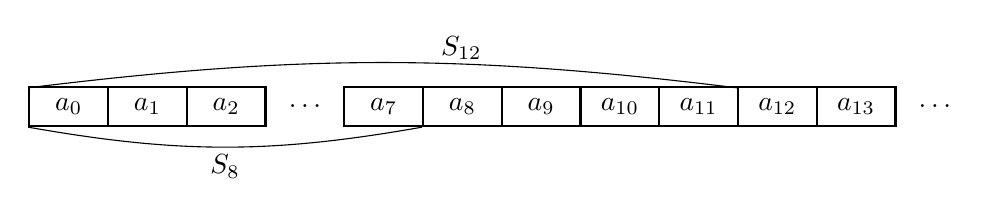
\begin{tikzpicture}[y=5mm]

\node[above right] (a0) at (0,0) [draw,thick,minimum width=1cm,minimum height=0.5cm] {$a_0$};
\node[above right] (a1) at (1,0) [draw,thick,minimum width=1cm,minimum height=0.5cm] {$a_1$};
\node[above right] (a2) at (2,0) [draw,thick,minimum width=1cm,minimum height=0.5cm] {$a_2$};
\node[above right] (a3) at (3,0) [thick,minimum width=1cm,minimum height=0.5cm] {$\ldots$};
\node[above right] (a7) at (4,0) [draw,thick,minimum width=1cm,minimum height=0.5cm] {$a_7$};
\node[above right] (a8) at (5,0) [draw,thick,minimum width=1cm,minimum height=0.5cm] {$a_8$};
\node[above right] (a9) at (6,0) [draw,thick,minimum width=1cm,minimum height=0.5cm] {$a_9$};
\node[above right] (a10) at (7,0) [draw,thick,minimum width=1cm,minimum height=0.5cm] {$a_{10}$};
\node[above right] (a11) at (8,0) [draw,thick,minimum width=1cm,minimum height=0.5cm] {$a_{11}$};
\node[above right] (a12) at (9,0) [draw,thick,minimum width=1cm,minimum height=0.5cm] {$a_{12}$};
\node[above right] (a13) at (10,0) [draw,thick,minimum width=1cm,minimum height=0.5cm] {$a_{13}$};
\node[above right] (a14) at (11,0) [thick,minimum width=1cm,minimum height=0.5cm] {$\ldots$};
\draw (0,0) to [out=-10,in=190] (5,0);
\node[] () at (2.5,-1) {$S_8$};
\draw (0,1) to [out=7,in=173] (9,1);
\node[] () at (5.5,2) {$S_{12}$};
\end{tikzpicture}
\end{center}

これを用いて,すべての区間の和を調べると求める最大値を得られる.

\begin{pbox}{A Traveler}{JOI 2009}
左右に行ったり来たりする旅程が与えられるので歩いた合計(の剰余)を求めよ.

\aojid{0549}  
\end{pbox}

考え方: 旅程の要素に「左に30個目の宿場に移動する」という指示があったと
して,30回の加算をすることは避けたい.そこで事前に各宿場について左端か
らの距離を事前に計算しておく.すると旅程の要素数である$M$回の加算で合計
の距離を求められる.

\subsection*{二次元の累積和}

同様の考え方は二次元にも応用できる:
補助変数を$S_{i+1,j+1} = \sum_{k=0}^i \sum_{l=0}^j a_{k,l}$ と定義する.
縦[i,i'), 横[j,j')の長方形領域の和は
$S_{i',j'} - S_{i,j'} - S_{i',j} + S_{i,j}$となる.(大きな長方形から余分にを引いて,引きすぎたものを調整する)
つまり,長方形領域の面積によらない定数回の演算で求めることができる.

\begin{center}
\begin{tikzpicture}

\draw (0,0) rectangle (6,4);
\draw[dotted] (2,0) -- (2,4);
\draw[dotted] (0,2.5) -- (6,2.5);
\node[below right] () at (0,4) [draw] {\small $a_{0,0}$};
\node[below right] () at (0,2.5) [draw] {\small $a_{i,0}$};
\node[below right] () at (2,2.5) [draw] {\small $a_{i,j}$};
\node[below right] () at (6,2.5) [draw,dotted] {\small $a_{i,j'}$};
\node[below right] () at (2,0) [draw,dotted] {\small $a_{i',j}$};
\node[below right] () at (6,0) [draw,dotted] {\small $a_{i',j'}$};
\node[] () at (1,1.25) {$C$};
\node[] () at (1,3.25) {$A$};
\node[] () at (4,1.25) {$D$};
\node[] () at (4,3.25) {$B$};
\node[] () at (10,2) {\vbox{\hbox{$A=S_{i,j}$}\hbox{$A+B=S_{i,j'}$}\hbox{$A+C=S_{i',j}$}\hbox{$A+B+C+D=S_{i',j'}$}}};
\end{tikzpicture}
\end{center}

\begin{psbox}{Maximum Sum Sequence II}{PC甲子園2003}
和が最大になる長方形領域を知りたい.

\aojid{0098}  
\end{psbox}

(この問題も縦横どちらかのmaximum subarray problemに変換することで,$O(N^3)$
で解ける.しかし,ストーリーの都合で全長方形区間を調べて$O(N^4)$で解く意図で掲載する)

\begin{pbox}{Planetary Exploration}{JOI 2010}
指定の長方形区域の資源の数を知りたい.

\aojid{0560}
\end{pbox}

\begin{pbox}{Coffee Central$\star$}{World Finals 2011}
カフェを開くのに最適な場所を知りたい.

\url{https://icpcarchive.ecs.baylor.edu/index.php?option=com_onlinejudge&Itemid=8&category=45&page=show_problem&problem=3133}
\end{pbox}

菱形の領域は45度回転させると扱いやすくなる場合がある.

\section{Binary Indexed Tree (Fenwick Tree)}

今度は処理の途中でデータ$a_i$の一部が変化する状況を考える.
前節のように補助変数$S$を使うと,質問には$O(1)$で回答できて効率が良いが
更新には$O(N)$かかってしまう.質問回答に$O(\log N)$のコストを許容することで,$O(\log N)$の更新を実現する手法を紹介する.(\pccbook[pp. 160--])

\begin{pbox}{Range Query - Range Sum Query}{AOJ}
区間の合計値を管理せよ  

\aojid{DSL_2_B}
\end{pbox}

\begin{center}
\begin{tikzpicture}[y=5mm]
\node[above right] (S8) at (0,6) [draw,thick,minimum width=8cm,minimum height=0.5cm] {$S_{1,8}$};
\node[above right] (S4) at (0,4) [draw,thick,minimum width=4cm,minimum height=0.5cm,fill=gray!15!] {$S_{1,4}$};
\node[above right] (S2) at (0,2) [draw,thick,minimum width=2cm,minimum height=0.5cm] {$S_{1,2}$};
\node[above right] (S6) at (4,2) [draw,thick,minimum width=2cm,minimum height=0.5cm,fill=gray!15!] {$S_{5,6}$};
\node[above right] (S1) at (0,0) [draw,thick,minimum width=1cm,minimum height=0.5cm] {$S_{1,1}$};
\node[above right] (S3) at (2,0) [draw,thick,minimum width=1cm,minimum height=0.5cm] {$S_{3,3}$};
\node[above right] (S5) at (4,0) [draw,thick,minimum width=1cm,minimum height=0.5cm] {$S_{5,5}$};
\node[above right] (S7) at (6,0) [draw,thick,minimum width=1cm,minimum height=0.5cm,fill=gray!15!] {$S_{7,7}$};
\node[right,color=iblue] at (7.9,6.5) {\small 8:1000};
\node[right,color=iblue] at (3.95,4.5) {\small 4:0100};
\node[right,color=iblue] at (1.95,2.5) {\small 2:0010};
\node[right,color=iblue] at (0.9,0.5) {\small 1:0001};
\node[right,color=iblue] at (5.95,2.5) {\small 6:0110};
\node[right,color=iblue] at (2.9,0.5) {\small 3:0011};
\node[right,color=iblue] at (4.9,0.5) {\small 5:0101};
\node[right,color=iblue] at (6.9,0.5) {\small 7:0111};
\end{tikzpicture}
\end{center}

まず図のような,2のべき乗の長さの区間に対する和を求めておく.ここで
$S_{i,j}$という表記は区間[i,j]の和とする.前節までと表記が異なり,$j$
を含む.また,管理対象の列は$a_1$と1から始まるとする.(0から始めること
もできるが,後に書くように微調整が必要である)

このような準備を行うと $x \ge 1 $にたいして$S_{1,x}$を$\log x$個までの
和として表現することができる.たとえば,$S_{1,7} =
S_{1,4}+S_{5,6}+S_{7,7}$である.
また,ある要素の値が変化した時には,最大$\log N$個の部分和を更新すれば
良い.たとえば,$a_7$が更新された時は,それを含む区間である$S_{7,7}$と$S_{1,7}$を更新する.

このようなデータを配列で管理するデータ構造がFenwick tree または Binary
indexed tree (BIT)である.青字で記した要素
番号(コロンの右側は2進表記)を用いると次のように管理することができる.
$n$番目の配列の要素\texttt{BIT[n]}には,左端$l$が$n$の最下位ビットを落とした数
+1でまた右端$r$が$n$であるような区間の和$S_{l,r}$を格納する.
したがって,$1$から$n$までの和は,まず\texttt{BIT[n]}を加え,カバーする
区間の左端$l$が$1$に到達するまで,現区間の$l-1$を右端とするような新しい区間を探して
足すことを繰り返せば良い.そのような区間は\texttt{n}の最下位ビットを落とすことで求められる.また$a_n$を更新する場合は\texttt{BIT[n]}の更新後に,その区間を含むブロックを(左端を減らさないように)右端を広げることで探すことを繰り返す.


\begin{cbox}
int BIT[1000010], bit_size;
void bit_init(int n) {
    fill(BIT, BIT+n, 0); 
    bit_size = n;
}
int bit_sum(int n) { // [1,n]の和
  int ans = 0;
  while (n > 0) { // 全体区間左端では1を一つだけ含むので最後は0になって終了
    ans += BIT[n];
    n &= n-1; // 最下位(右端)の1を落とす: 左に移動
  }
  return ans;
}
void bit_add(int n, int v) { // n番目の要素にvに加える
  while (n <= bit_size) {
    BIT[n] += v;
    n += n & (-n); // 最下位(右端)の1を繰り上げる
  }
}  
\end{cbox}

\paragraph{参考: 0-indexの場合}
\begin{center}
\begin{tikzpicture}[y=5mm]
\node[above right] (S8) at (0,6) [draw,thick,minimum width=8cm,minimum height=0.5cm] {$S_{0,7}$};
\node[above right] (S4) at (0,4) [draw,thick,minimum width=4cm,minimum height=0.5cm] {$S_{0,3}$};
\node[above right] (S2) at (0,2) [draw,thick,minimum width=2cm,minimum height=0.5cm] {$S_{0,1}$};
\node[above right] (S6) at (4,2) [draw,thick,minimum width=2cm,minimum height=0.5cm] {$S_{4,5}$};
\node[above right] (S1) at (0,0) [draw,thick,minimum width=1cm,minimum height=0.5cm] {$S_{0,0}$};
\node[above right] (S3) at (2,0) [draw,thick,minimum width=1cm,minimum height=0.5cm] {$S_{2,2}$};
\node[above right] (S5) at (4,0) [draw,thick,minimum width=1cm,minimum height=0.5cm] {$S_{4,4}$};
\node[above right] (S7) at (6,0) [draw,thick,minimum width=1cm,minimum height=0.5cm] {$S_{6,6}$};
\node[right,color=iblue] at (7.9,6.5) {\small 7:111};
\node[right,color=iblue] at (3.95,4.5) {\small 3:011};
\node[right,color=iblue] at (1.95,2.5) {\small 1:001};
\node[right,color=iblue] at (0.9,0.5) {\small 0:000};
\node[right,color=iblue] at (5.95,2.5) {\small 5:101};
\node[right,color=iblue] at (2.9,0.5) {\small 2:010};
\node[right,color=iblue] at (4.9,0.5) {\small 4:100};
\node[right,color=iblue] at (6.9,0.5) {\small 6:110};
\end{tikzpicture}
\end{center}

\begin{itemize}
\setlength{\itemsep}{0pt}
\item[和:]  \texttt{n = (n \& (n + 1)) - 1 } $(n\ge 0)$ 右に0のある1を繰り下げる
\item[更新:]  \texttt{n |= n + 1 } $(n<\text{size})$  一番右の0を1に
\end{itemize}

\begin{pbox}{引越し}{夏合宿2012}
小さい順に並べ替えるのに必要な体力の合計を求める.

\aojid{2431}
\end{pbox}

全部並べ替えると1からNまでの総和なので,それから並べ替えなくて良い(=昇順の)部分
列の重さの総和の最大値を引けば良い.

$i$番目の数字$x_i$で終わるような昇順の部分列の重さの和の最大値を$A_i$と表記すると,
$$
A_i = x_i + \max_{j<i,\, x_j<x_i} A_j
$$
なので,数列を左から見てゆくと順に求められる.ここで$i$より小さい$j$について最大値を逐一調べると時間がかかるので,$x_i$をキーとしたBITを使って効率良く処理を行う.

\begin{cbox}
long long N, x;
int main() {
    cin >> N;
    bit_init(N+1);
    for (int i=0; i<N; ++i) {
        cin >> x;
        long long cost = // xまでの最大値
        ... // xまでの最大値を cost+xに更新
    }
    cout << (1+N)*N/2 - bit_max(N) << endl;
}
\end{cbox}

\begin{rbox}
N = gets.to_i
X = gets.split(' ').map{|s| s.to_i}

tree = BIT_Max.new(N+1)
X.each {|x|
  cost = ... // xまでの最大値
  ... // xまでの最大値を cost+xに更新
}
puts (1+N)*N/2 - tree.max(N)  
\end{rbox}

区間の和を管理するBITの代わりに,
先頭からの区間$[1,n]$の最大値を持つデータ構造を考える.

\begin{cbox}
long long BIT[100010], bit_size; // long longは64bit整数.
void bit_init(int n) {
    fill(BIT, BIT+n, 0); 
    bit_size = n;
}
long long bit_max(int n) { // [1,n]の最大値
    long long ans = 0;
    while (n > 0) {
        ans = max(ans, BIT[n]);
        n &= n-1;
    }
    return ans;
}
void bit_setmax(int n, long long v) { // \# [1,n]の最大値をvに更新する
    while (n < bit_size) {
        BIT[n] = max(BIT[n], v);
        n += n & (-n);
    }
}  
\end{cbox}

\begin{rbox}
class BIT_Max
  # 1-index
  def initialize(n)
    @array = Array.new(n+1, 0)
  end
  def max(n) # [1,n]の最大値
    ans = 0
    while n > 0
      ans = @array[n] if ans < @array[n]
      n &= n-1
    end
    ans
  end
  def setmax(n, v) # [1,n]の最大値をvに更新する
    while n < @array.size
      @array[n] = v if @array[n] < v
      n += n & (-n)
    end
  end
end
\end{rbox}

\section{Segment TreeとRange Minimum Query}\label{section:RMQ}

次に区間の最小値や最大値について考えてみる.
区間[i,j]の最小値は,残念ながら,区間[0,i]の最小値や区間[0,j]の最小値からは求めることができない.そこでもう少しデータの豊富なSegment Treeを用いる.
(\pccbook[pp.~154--]).

\begin{center}
\begin{tikzpicture}[y=5mm]
\node[above right] (S0) at (0,6) [draw,thick,minimum width=8cm,minimum height=0.5cm] {$S_{0,7}$};
\node[above right] (S1) at (0,4) [draw,thick,minimum width=3.9cm,minimum height=0.5cm] {$S_{0,3}$};
\node[above right] (S2) at (4,4) [draw,thick,minimum width=4cm,minimum height=0.5cm] {$S_{4,7}$};
\node[above right] (S3) at (0,2) [draw,thick,minimum width=1.9cm,minimum height=0.5cm] {$S_{0,1}$};
\node[above right] (S4) at (2,2) [draw,thick,minimum width=1.9cm,minimum height=0.5cm,fill=gray!15!] {$S_{2,3}$};
\node[above right] (S5) at (4,2) [draw,thick,minimum width=1.9cm,minimum height=0.5cm,fill=gray!15!] {$S_{4,5}$};
\node[above right] (S6) at (6,2) [draw,thick,minimum width=2cm,minimum height=0.5cm] {$S_{6,7}$};
\node[above right] (S7) at (0,0) [draw,thick,minimum width=.9cm,minimum height=0.5cm] {$S_{0,0}$};
\node[above right] (S8) at (1,0) [draw,thick,minimum width=.9cm,minimum height=0.5cm,fill=gray!15!] {$S_{1,1}$};
\node[above right] (S9) at (2,0) [draw,thick,minimum width=.9cm,minimum height=0.5cm] {$S_{2,2}$};
\node[above right] (S10) at (3,0) [draw,thick,minimum width=.9cm,minimum height=0.5cm] {$S_{3,3}$};
\node[above right] (S11) at (4,0) [draw,thick,minimum width=.9cm,minimum height=0.5cm] {$S_{4,4}$};
\node[above right] (S12) at (5,0) [draw,thick,minimum width=.9cm,minimum height=0.5cm] {$S_{5,5}$};
\node[above right] (S13) at (6,0) [draw,thick,minimum width=.9cm,minimum height=0.5cm,fill=gray!15!] {$S_{6,6}$};
\node[above right] (S14) at (7,0) [draw,thick,minimum width=1cm,minimum height=0.5cm] {$S_{7,7}$};
\node[color=icyan] at (7.8,6.5) {0};
\node[color=icyan] at (3.6,4.5) {1};
\node[color=icyan] at (7.8,4.5) {2};
\node[color=icyan] at (1.6,2.5) {3};
\node[color=icyan] at (3.6,2.5) {4};
\node[color=icyan] at (5.6,2.5) {5};
\node[color=icyan] at (7.8,2.5) {6};
\node[color=icyan] at (0.5,-0.5) {7};
\node[color=icyan] at (1.5,-0.5) {8};
\node[color=icyan] at (2.5,-0.5) {9};
\node[color=icyan] at (3.5,-0.5) {10};
\node[color=icyan] at (4.5,-0.5) {11};
\node[color=icyan] at (5.5,-0.5) {12};
\node[color=icyan] at (6.5,-0.5) {13};
\node[color=icyan] at (7.5,-0.5) {14};
\end{tikzpicture}
\end{center}

図のような全区間を根として番号0とする完全二分木で,各区間のデータを保
持する.葉以外の各区間は2つの子を持ち,左の子が親の区間の左半分,右の
子が残りを担当する.
たとえば,区間[2,6]の最小値は図の灰色部分のように,$\min(S_{1,2},S_{2,3},S_{4,5},S_{6,6})$で求められる.どのような区間をとっても,調べる箇所は各深さ毎に最大2までである.


この実装では,ある\texttt{id}について, 左の子は\texttt{id*2+1},右の子は\texttt{id*2+2},親は\texttt{(id-1)/2}である.
元の配列$a_i$の長さを$N$とすると,$N$が2のべき乗なら$2N$の領域を,そうでなければ最大$4N$の領域を使用する.

また,根付き木の最小共通祖先
LCA (least/lowest common ancestor)を,深さ優先探索の訪問時刻に対するRMQとして,計算することもできる.
\pccbook[pp.~292--]

\begin{pbox}{Range Query - Range Minimum Query}{AOJ}
区間の最小値を管理せよ

\aojid{DSL_2_A}
\end{pbox}

\begin{pbox}{Balanced Lineup}{USACO 2007 January Silver}
牛が並んでいる. 区間[a,b]で身長が最大の牛と最小の牛の差は?

\url{http://poj.org/problem?id=3264}
\end{pbox}

scanf必要.

\begin{pbox}{Drawing Lots$\star$}{UTPC2009}
あみだくじについて,選ばれた場所がアタリとなるように横線の数を追加するとして,その最小本数を求めよ.

  \aojid{2192}
\end{pbox}

\begin{pbox}{Distance Queries$\star$}{USACO 2004 February}

農場間2点の道のりを求める

\url{http://poj.org/problem?id=1986}
\end{pbox}


\begin{pbox}{Apple Tree$\star$}{POJ Monthly--2007.08.05}

りんごの数を数える

\url{http://poj.org/problem?id=3321}
\end{pbox}

\end{versionbeta}

 \begin{versionalpha}
\chapter{グラフ(4) ネットワークフローとマッチング}

\section{Stable Matching (安定結婚問題)}

二つのグループAとBがあり,その間の対応を取る問題を考える.AとBには,研
修医と病院の受け入れ,男女の結婚,生産物と工場などの例を想定する.初め
に扱うのは,AとBに同数$N$の要素があり,AとBから要素を一つづつ選んでペア
を作り,要素が重複しない$N$のペア(\textbf{マッチング}\footnote{グラフでは,互いに隣接しない(\textbf{独立}な)辺の集合を\textbf{マッチング}と呼ぶ.})を作成する問題で
ある.

たとえば結婚が題材の場合は,A, Bが男性と女性となる.ここでは,各
個人が相手とする希望順位を示すリスト持ち,リストには異性の全員が列挙さ
れているとする.この設定では,ある意味で希望を満たす安定なペアを全員に
作ることができる.ここで安定とは,「現在のペアを崩して新たなペアを作っ
た時に,男性も女性も現在のペアより望ましい状況」になら*ない*ことを言う.

\begin{itembox}{安定と不安定の例}
  1名づつ募集する職種$A,B$と応募者$a,b$のそれぞれが選好順位を決めたと
  する.以下のような例では,いずれも$Aa$をペアにしていない場合,現ペアを崩して$Aa$を組にすると$A$も$a$も現在のペアより望ましい状況になる.

  \begin{center}
  \begin{tabular}{cccc|lll}
    \multicolumn{4}{l|}{希望順} & 安定 & 不安定 &不安定の理由\\
    $A$ & $B$ & $a$ & $b$ \\\hline
    $ab$&  $ba$& $AB$& $BA$   & ($Aa, Bb$) & ($Ab, Ba$) & 第一希望が一致\\
    $ab$&  $ab$& $AB$& $BA$   & ($Aa, Bb$) & ($Ab, Ba$)
    & $B$にとっては第一志望だが不安定\\
    $ab$&  $ab$& $AB$& $AB$   & ($Aa, Bb$) & ($Ab, Ba$)& $B, b$にとっては第一志望だが不安定
  \end{tabular}
  \end{center}
\end{itembox}

この問題は,下記のように(1)仮のペアを決める(2)より優先順位の高いペアが
後からできたらそれで置き換えることを繰り返して解くことができる(Gale–Shapley)
.
\begin{cbox}
while 全員がペアになるまで
 独身の男性を一人選び m とする
  mの希望リストで,「まだ断られていない中で」最上位の女性をfとする
  if f が独身
    mとfをペアにする
  else if f はm'と現在ペアである
    if fにとってm'がmより好み
      m は独身のまま
    else
      mとfをペアにする
      m'は独身に戻る
    end
  end
end  
\end{cbox}

\medskip

この問題は,上記のように(1)仮のペアを決める(2)より優先順位の高いペアが
できたらそれで置き換えることを繰り返して解くことができる.男性と女性は
対称なので入れ替えても安定な解を得ることができる.その場合,安定な解が
複数ある場合にどちら側の希望が優先されるかに違いが表れる.表記を
短くするために,ペアがない状態を独身と表記した.


\begin{pbox}{The Stable Marriage Problem}{Southeastern Europe 2007}

男女$N$人づつの希望リストが与えられるので,安定なマッチングを男性の希望優先で作成せよ.

男性はアルファベット大文字一文字,女性はアルファベット小文字一文字で表
される.各希望には$N$人が列挙されている.出力は,男性の名前順で処理する.

\url{http://poj.org/problem?id=3487}
\end{pbox}

各男性や女性が名前で与えられるので,0..Nなどの数値で与えられる場合よりも,多少複雑になる.
ここではアルファベット一文字は$[0,127]$の数値と等価であることを利用して,数字だと思って扱う.
男性\texttt{'a'}さんの好みのリストを\texttt{pref\_m['a']}の先頭$N$文字
で表し,同様に女性\texttt{'A'}さんの好みのリストを
\texttt{pref\_m['A']}で表す.
すなわち男性\texttt{'a'}さんにとって,最も好みの女性は
\texttt{pref\_m['a'][0]}で,その次は\texttt{pref\_m['a'][1]}などと表さ
れる.
表の使わない部分はNULL文字(C++では0から自動で変換される)をつめておく.


\begin{cbox}
#include <algorithm>
// 最初のsampleではpref\_m['a'] は BAC... (先頭N文字だけ使い,他はnull)
char pref_m[256][256]={{0}}, pref_f[256][256]={{0}},;

// 女性f が,男性aを男性bより好む場合に真
bool better(char f, char a, char b) { 
  int orda = find(pref_f[f], pref_f[f]+27, a) - pref_f[f]; // a のリスト内の順位
  int ordb = find(pref_f[f], pref_f[f]+27, b) - pref_f[f]; // b
  return orda < ordb;
}
\end{cbox}

続いて入出力を作る.少し複雑なので,下記のサンプルの隅々まで理解していなくても,動作が確認できれば問題ない.\texttt{scanf(" \%c",c)}は空白を読み飛ばして1文字読む文法.


\begin{cbox}
#include <cstdio>
#include <iostream>
#include <string>
using namespace std;
int T, N;
int main() {
    scanf("
    for (int t=0; t<T; ++t) {
        scanf("
        string name_m, name_f;
        char c;
        for (int i=0; i<N; ++i) {
            scanf(" 
            name_m += c;
        }
        for (int i=0; i<N; ++i) {
            scanf(" 
            name_f += c;
        }
        sort(name_m.begin(), name_m.end());
        
        for (int i=0; i<N; ++i) {
            scanf(" 
            scanf("
        }
        for (int i=0; i<N; ++i) {
            scanf(" 
            scanf("
        }
        if (t>0) puts("");
        // 問題を解く前に,pref\_m や pref\_fを出力しよう
        for (int i=0; i<N; ++i)
            cout << name_m[i] << pref_m[name_m[i]] << endl;
        for (int i=0; i<N; ++i)
            cout << name_f[i] << pref_f[name_f[i]] << endl;
        // つづいてこの辺でsolve()関数を呼ぶように組み合わせる
    }
}
\end{cbox}


\begin{center}
  \begin{tabular}{l@{\hspace{1.5cm}}l@{\hspace{1.5cm}}l}
      \begin{tikzpicture}[node distance=15mm]
        \node[city] (a)              {$a$};
        \node[city] (b) [right of=a] {$b$};
        \node[city] (c) [right of=b] {$c$};

        \node[city] (A) [below of=a] {$A$};
        \node[city] (B) [right of=A] {$B$};
        \node[city] (C) [right of=B] {$C$};

        \path[->,thick,draw=red] (a) edge (B);
      \end{tikzpicture}
&
      \begin{tikzpicture}[node distance=15mm]
        \node[city] (a)              {$a$};
        \node[city] (b) [right of=a] {$b$};
        \node[city] (c) [right of=b] {$c$};

        \node[city] (A) [below of=a] {$A$};
        \node[city] (B) [right of=A] {$B$};
        \node[city] (C) [right of=B] {$C$};

        \path[->,thick] (a) edge (B);
        \path[->,dotted,draw=red] (b) edge (B);
      \end{tikzpicture}

&
      \begin{tikzpicture}[node distance=15mm]
        \node[city] (a)              {$a$};
        \node[city] (b) [right of=a] {$b$};
        \node[city] (c) [right of=b] {$c$};

        \node[city] (A) [below of=a] {$A$};
        \node[city] (B) [right of=A] {$B$};
        \node[city] (C) [right of=B] {$C$};

        \path[->,thick,draw=red] (b) edge (B);
      \end{tikzpicture}
\\
(1) aの第一希望はB & (2) bの第一希望はB (競合) & (3) Bはbをaより好む \\
      \begin{tikzpicture}[node distance=15mm]
        \node[city] (a)              {$a$};
        \node[city] (b) [right of=a] {$b$};
        \node[city] (c) [right of=b] {$c$};

        \node[city] (A) [below of=a] {$A$};
        \node[city] (B) [right of=A] {$B$};
        \node[city] (C) [right of=B] {$C$};

        \path[->,thick,draw=red] (a) edge (A);
        \path[->,thick] (b) edge (B);
      \end{tikzpicture}
&
      \begin{tikzpicture}[node distance=15mm]
        \node[city] (a)              {$a$};
        \node[city] (b) [right of=a] {$b$};
        \node[city] (c) [right of=b] {$c$};

        \node[city] (A) [below of=a] {$A$};
        \node[city] (B) [right of=A] {$B$};
        \node[city] (C) [right of=B] {$C$};

        \path[->,thick] (a) edge (A);
        \path[->,thick] (b) edge (B);
        \path[->,dotted,draw=red] (c) edge (A);
      \end{tikzpicture}
&
      \begin{tikzpicture}[node distance=15mm]
        \node[city] (a)              {$a$};
        \node[city] (b) [right of=a] {$b$};
        \node[city] (c) [right of=b] {$c$};

        \node[city] (A) [below of=a] {$A$};
        \node[city] (B) [right of=A] {$B$};
        \node[city] (C) [right of=B] {$C$};

        \path[->,thick] (a) edge (A);
        \path[->,thick] (b) edge (B);
        \path[->,thick,draw=red] (c) edge (C);
      \end{tikzpicture}
\\
(4) aの次の希望はA & (5) cの希望もA (競合) & (6) Aはaを選びcはCに
  \end{tabular}
The Stable Marriage Problem: 最初のサンプルでの動作例
\end{center}


続いて,アルゴリズムを実装する.
男性\texttt{'a'}さんの現在のペアを\texttt{m2f['a']}で表す(居ない場合はNULL文字).
同様に女性\texttt{'A'}さんの現在のペアを\texttt{f2m['A']}で表す.

男性\texttt{'a'}さんが,自分のリスト内の何人目までプロポーズした状況かを\texttt{proposed['a']}で管理する.

\begin{cbox}
void solve(string name_m, string name_f) {
    char m2f[256]={0}, f2m[256]={0};
    int proposed[256]={0};
    int man_id = 0; // 何人目の男性
    while (true) {
        char man = name_m[man_id]; // 男性の名前
        if (m2f[man]) { // 割り当て済
            ++man_id; // 次の人へ
            if (man_id == N) break;
            continue;
        }
        // manさんには今ペアが以内
        while (!m2f[man]) {
            char f =  ... // manの「次の優先順位」の女性を選ぶ
            ... // manの「次の優先順位」を+1しておく
            char mate = ... // fさんの現在のペア
            if (! mate || better(f, man, mate)) {
                if (mate) m2f[mate] = 0; // mateとfのペア解消
                ... // manとfがペア成立をmf2とf2mに記録
                man_id = 0; // 初めから見直す
            }
        }
    }
    for (int i=0; i<N; ++i)
        printf("
}
\end{cbox}

\section{二部グラフのマッチング}


二部グラフで,大きさが最大のマッチングを求める問題を考えてみよう.
前節と似た設定の問題であるが,希望順位がないことと全員をペアにできると
は限らないことが異なる.仮のペアを決めて,必要に応じて割り当て直すこと
は前節と同様であるが,その割り当て直しをおこなって良いかどうかの判定に
は再帰を用いる必要がある.(\pccbook[pp.~195--])

\begin{psbox}{Matching - Bipartite Matching}{AOJ}
  
\aojid{GRL_7_A}
\end{psbox}

サンプル入力1での動作例を示す.

\begin{center}
  \begin{tabular}{l@{\hspace{1.5cm}}l}
      \begin{tikzpicture}[node distance=15mm]
        \node[city] (a)              {$0$};
        \node[city] (b) [right of=a] {$1$};
        \node[city] (c) [right of=b] {$2$};

        \node[city] (A) [below of=a] {$0$};
        \node[city] (B) [right of=A] {$1$};
        \node[city] (C) [right of=B] {$2$};
        \node[city] (D) [right of=C] {$3$};

        \path[draw=gray,thick] (a) edge (A);
        \path[draw=gray,thick] (a) edge (C);
        \path[draw=gray,thick] (a) edge (D);
        \path[draw=gray,thick] (b) edge (B);
        \path[draw=gray,thick] (c) edge (B);
        \path[draw=gray,thick] (c) edge (C);
      \end{tikzpicture}
&
      \begin{tikzpicture}[node distance=15mm]
        \node[vcity] (a)              {$0$};
        \node[city] (b) [right of=a] {$1$};
        \node[city] (c) [right of=b] {$2$};

        \node[ccity] (A) [below of=a] {$0$};
        \node[city] (B) [right of=A] {$1$};
        \node[city] (C) [right of=B] {$2$};
        \node[city] (D) [right of=C] {$3$};

        \path[draw=red,thick] (a) edge (A);
        \path[draw=gray,thick] (a) edge (C);
        \path[draw=gray,thick] (a) edge (D);
        \path[draw=gray,thick] (b) edge (B);
        \path[draw=gray,thick] (c) edge (B);
        \path[draw=gray,thick] (c) edge (C);
      \end{tikzpicture}\\
  初期状態 & 上の0から一つ仮ペアを作る\\
      \begin{tikzpicture}[node distance=15mm]
        \node[vcity] (a)              {$0$};
        \node[vcity] (b) [right of=a] {$1$};
        \node[city] (c) [right of=b] {$2$};

        \node[ccity] (A) [below of=a] {$0$};
        \node[ccity] (B) [right of=A] {$1$};
        \node[city] (C) [right of=B] {$2$};
        \node[city] (D) [right of=C] {$3$};

        \path[draw=blue,thick] (a) edge (A);
        \path[draw=gray,thick] (a) edge (C);
        \path[draw=gray,thick] (a) edge (D);
        \path[draw=red,thick] (b) edge (B);
        \path[draw=gray,thick] (c) edge (B);
        \path[draw=gray,thick] (c) edge (C);
      \end{tikzpicture}
&
      \begin{tikzpicture}[node distance=15mm]
        \node[vcity] (a)              {$0$};
        \node[vcity] (b) [right of=a] {$1$};
        \node[vcity] (c) [right of=b] {$2$};

        \node[ccity] (A) [below of=a] {$0$};
        \node[ccity] (B) [right of=A] {$1$};
        \node[city] (C) [right of=B] {$2$};
        \node[city] (D) [right of=C] {$3$};

        \path[draw=blue,thick] (a) edge (A);
        \path[draw=gray,thick] (a) edge (C);
        \path[draw=gray,thick] (a) edge (D);
        \path[draw=blue,thick] (b) edge (B);
        \path[draw=red,thick] (c) edge (B);
        \path[draw=gray,thick] (c) edge (C);
      \end{tikzpicture}\\
上の1から仮ペアを作る & 上の2から仮ペアを作ろうとすると衝突
\\
      \begin{tikzpicture}[node distance=15mm]
        \node[vcity] (a)              {$0$};
        \node[vcity] (b) [right of=a] {$1$};
        \node[vcity] (c) [right of=b] {$2$};

        \node[ccity] (A) [below of=a] {$0$};
        \node[ccity] (B) [right of=A] {$1$};
        \node[city] (C) [right of=B] {$2$};
        \node[city] (D) [right of=C] {$3$};

        \path[draw=blue,thick] (a) edge (A);
        \path[draw=gray,thick] (a) edge (C);
        \path[draw=gray,thick] (a) edge (D);
        \path[draw=blue,dotted] (b) edge (B);
        \path[draw=red,thick] (c) edge (B);
        \path[draw=gray,thick] (c) edge (C);
      \end{tikzpicture}
&
      \begin{tikzpicture}[node distance=15mm]
        \node[vcity] (a)              {$0$};
        \node[vcity] (b) [right of=a] {$1$};
        \node[vcity] (c) [right of=b] {$2$};

        \node[ccity] (A) [below of=a] {$0$};
        \node[ccity] (B) [right of=A] {$1$};
        \node[city] (C) [right of=B] {$2$};
        \node[city] (D) [right of=C] {$3$};

        \path[draw=blue,thick] (a) edge (A);
        \path[draw=gray,thick] (a) edge (C);
        \path[draw=gray,thick] (a) edge (D);
        \path[draw=blue,thick] (b) edge (B);
        \path[draw=gray,dotted] (c) edge (B);
        \path[draw=red,thick] (c) edge (C);
      \end{tikzpicture}
\\
1のペアを組み替えても上1が孤立 & 1の仮ペアを元に戻して2は別のペアに
  \end{tabular}
\end{center}

もう少し複雑な,割り当て直しが発生する例でも確認しよう.
\begin{alltt}
3 3 6
0 0
0 1
0 2
1 0
1 1
2 0
\end{alltt}

\begin{center}
  \begin{tabular}{l@{\hspace{1.5cm}}l@{\hspace{1.5cm}}l}
      \begin{tikzpicture}[node distance=15mm]
        \node[city] (a)              {$0$};
        \node[city] (b) [right of=a] {$1$};
        \node[city] (c) [right of=b] {$2$};

        \node[city] (A) [below of=a] {$0$};
        \node[city] (B) [right of=A] {$1$};
        \node[city] (C) [right of=B] {$2$};

        \path[draw=gray,thick] (a) edge (A);
        \path[draw=gray,thick] (a) edge (B);
        \path[draw=gray,thick] (a) edge (C);
        \path[draw=gray,thick] (b) edge (A);
        \path[draw=gray,thick] (b) edge (B);
        \path[draw=gray,thick] (c) edge (A);
      \end{tikzpicture}
      &
      \begin{tikzpicture}[node distance=15mm]
        \node[vcity] (a)              {$0$};
        \node[city] (b) [right of=a] {$1$};
        \node[city] (c) [right of=b] {$2$};

        \node[ccity] (A) [below of=a] {$0$};
        \node[city] (B) [right of=A] {$1$};
        \node[city] (C) [right of=B] {$2$};

        \path[draw=red,thick] (a) edge (A);
        \path[draw=gray,thick] (a) edge (B);
        \path[draw=gray,thick] (a) edge (C);
        \path[draw=gray,thick] (b) edge (A);
        \path[draw=gray,thick] (b) edge (B);
        \path[draw=gray,thick] (c) edge (A);
      \end{tikzpicture}
&
      \begin{tikzpicture}[node distance=15mm]
        \node[vcity] (a)              {$0$};
        \node[vcity] (b) [right of=a] {$1$};
        \node[city] (c) [right of=b] {$2$};

        \node[ccity] (A) [below of=a] {$0$};
        \node[city] (B) [right of=A] {$1$};
        \node[city] (C) [right of=B] {$2$};

        \path[draw=red,thick] (a) edge (A);
        \path[draw=gray,thick] (a) edge (B);
        \path[draw=gray,thick] (a) edge (C);
        \path[draw=red,thick] (b) edge (A);
        \path[draw=gray,thick] (b) edge (B);
        \path[draw=gray,thick] (c) edge (A);
      \end{tikzpicture}\\
  初期状態 & 上の0から一つ仮ペアを作る & 上の1の仮ペアは$\cdots$\\
      \begin{tikzpicture}[node distance=15mm]
        \node[vcity] (a)              {$0$};
        \node[vcity] (b) [right of=a] {$1$};
        \node[city] (c) [right of=b] {$2$};

        \node[ccity] (A) [below of=a] {$0$};
        \node[ccity] (B) [right of=A] {$1$};
        \node[city] (C) [right of=B] {$2$};

        \path[draw=red,dotted] (a) edge (A);
        \path[draw=red,thick] (a) edge (B);
        \path[draw=gray,thick] (a) edge (C);
        \path[draw=red,thick] (b) edge (A);
        \path[draw=gray,thick] (b) edge (B);
        \path[draw=gray,thick] (c) edge (A);
      \end{tikzpicture}
&
      \begin{tikzpicture}[node distance=15mm]
        \node[vcity] (a)              {$0$};
        \node[vcity] (b) [right of=a] {$1$};
        \node[vcity] (c) [right of=b] {$2$};

        \node[ccity] (A) [below of=a] {$0$};
        \node[ccity] (B) [right of=A] {$1$};
        \node[city] (C) [right of=B] {$2$};

        \path[draw=red,dotted] (a) edge (A);
        \path[draw=red,thick] (a) edge (B);
        \path[draw=gray,thick] (a) edge (C);
        \path[draw=red,thick] (b) edge (A);
        \path[draw=gray,thick] (b) edge (B);
        \path[draw=red,thick] (c) edge (A);
      \end{tikzpicture}
&
      \begin{tikzpicture}[node distance=15mm]
        \node[vcity] (a)              {$0$};
        \node[vcity] (b) [right of=a] {$1$};
        \node[vcity] (c) [right of=b] {$2$};

        \node[ccity] (A) [below of=a] {$0$};
        \node[ccity] (B) [right of=A] {$1$};
        \node[city] (C) [right of=B] {$2$};

        \path[draw=red,dotted] (a) edge (A);
        \path[draw=red,thick] (a) edge (B);
        \path[draw=gray,thick] (a) edge (C);
        \path[draw=red,dotted] (b) edge (A);
        \path[draw=gray,thick] (b) edge (B);
        \path[draw=red,thick] (c) edge (A);
      \end{tikzpicture}\\
上の0の仮ペアを組み直す & 上2の仮ペアは & 下0を組み直し\\
      \begin{tikzpicture}[node distance=15mm]
        \node[vcity] (a)              {$0$};
        \node[vcity] (b) [right of=a] {$1$};
        \node[vcity] (c) [right of=b] {$2$};

        \node[ccity] (A) [below of=a] {$0$};
        \node[ccity] (B) [right of=A] {$1$};
        \node[city] (C) [right of=B] {$2$};

        \path[draw=red,dotted] (a) edge (A);
        \path[draw=red,dotted] (a) edge (B);
        \path[draw=gray,thick] (a) edge (C);
        \path[draw=red,dotted] (b) edge (A);
        \path[draw=red,thick] (b) edge (B);
        \path[draw=red,thick] (c) edge (A);
      \end{tikzpicture}
&
      \begin{tikzpicture}[node distance=15mm]
        \node[vcity] (a)              {$0$};
        \node[vcity] (b) [right of=a] {$1$};
        \node[vcity] (c) [right of=b] {$2$};

        \node[ccity] (A) [below of=a] {$0$};
        \node[ccity] (B) [right of=A] {$1$};
        \node[city] (C) [right of=B] {$2$};

        \path[draw=red,dotted] (a) edge (A);
        \path[draw=red,dotted] (a) edge (B);
        \path[draw=red,thick] (a) edge (C);
        \path[draw=red,dotted] (b) edge (A);
        \path[draw=red,thick] (b) edge (B);
        \path[draw=red,thick] (c) edge (A);
      \end{tikzpicture}\\
上1を組み直し & 上0を組み直し & 
  \end{tabular}
\end{center}

入力例
\begin{cbox}
int X, Y, E, x, y; // 問題入力
bool D[110][110] = {}; // 隣接行列
int main() {
  cin >> X >> Y >> E;
  for (int i=0; i<E; ++i) {
    cin >> x >> y;
    D[x][y] = true;
  }
  // ここで計算する
}
\end{cbox}

計算部分
\begin{cbox}
int PY[110]; // Yの現在のペア
bool V[110];
bool match(int x) {
  if (x<0) return true;
  if (V[x]) return false;
  V[x] = true;
  for (int y=0; y<Y; ++y) {
    if (!D[x][y]) continue;
    if (match(PY[y])) {
      PY[y] = x;
      return true;
    }
  }
  return false;
}
int main() {
  ... // 入力は終わっているとする
  fill(PY, PY+Y, -1); // 現在のペアを初期化
  int count = 0; // マッチした数
  for (int x=0; x<X; ++x) { // X側から順に試す
    fill(V, V+X, false);
    if (match(x)) ++count; // xを起点の割り当てが一つでも成功すれば
  }
  ... // 出力
}
\end{cbox}

\begin{pbox}{Cards$\star$}{国内予選2009}

青と赤のカードをペアにしてとりのぞく。最大何枚取り除けるか  

\aojid{1163}
\end{pbox}

\begin{cbox}
int main() {
    while (入力) {
       // 全ての赤いカードのペアを無し(-1)に
       P[赤全部] = -1;
       // C[青][赤]=1 (ペアに出来る場合), C[青][赤]=0 (できない場合)と
       設定
       for (全ての青いカード:青)
           for (全ての赤いカード: 赤)
               C[青][赤] = (__gcd(B[青], R[赤]) >= 2);
       // 青を一枚づつマッチ
       count = 0;
       for (全ての青いカード:青) {
           V[赤全部] = false;
           if (match(青)) ++count;
       }
       countが答え;
    }
}
\end{cbox}

\begin{cbox}
// V[赤] .. true ならカード赤に新しい割り当て先はない, falseなら不明
// P[赤] .. カード赤とペアになっている青いカード番号, 割り当てなしなら-1
bool match(int 青) { // 今までのペア数を減らさずに青をペアにできるか?
    if (青 < 0) return true;
    for (全ての赤いカード: 赤) {
       if (``青''と''赤''はペアに出来ない || V[赤]が真) continue;
       V[赤] = true;
       if (match(P[赤])) { // P[赤]に今までとは別のペアを見つけられたら
         P[赤] = 青; // ``赤''の新しいペアは青
         return true;
       }
    }
    return false;
}
\end{cbox}

\begin{pbox}{Defend the Bases$\star$}{夏合宿2009}
部隊を移動させて,基地を全部守る.(明記されていないが部隊の数は十分あるよう)
  
\aojid{2161}
\end{pbox}

\section{様々な対応付け}

\begin{pbox}{Skiers$\star$}{9th Polish Olympiad in Informatics}
スキー場の全てのコースを点検するために、何回頂上に登る必要があるかを求めよ。

\url{http://main.edu.pl/en/archive/oi/9/nar} 
\end{pbox}

\begin{pbox}{Dangerous Tower}
高い塔を作りたい

\aojid{2293}
  \end{pbox}


\begin{pbox}{Travel Agency$\star\star$}{Algorithmic Engagements 2006}
一緒に旅行に行きたい人と行きたくない人(!)が数値でモデル化されている。
最適な旅行メンバーを求めよ。

\url{http://main.edu.pl/en/archive/pa/2006/biu}
\end{pbox}

\begin{pbox}{Matching$\star\star$}{Central European Olympiad in Informatics 2011}
一連のロゴを貼れる,連続するビル群を選ぶ.

\url{http://main.edu.pl/en/archive/ceoi/2011/mat}
\end{pbox}

この問題はどちらかというと文字列のマッチングに近い.

\begin{pbox}{Ice Skates}{}
スケート靴の割り当て
  
\url{http://main.edu.pl/en/archive/oi/16/lyz}
\end{pbox}
\end{versionalpha}
 \begin{versionalpha}
\chapter{組み合わせゲーム}



\section{不偏ゲームと}

Combinatorial gamesの一部は比較的出題例があるようである.Nimの解き方や,
Grundy 数(\pccbook[pp.~272-]),surreal number
(\url{https://www.youtube.com/watch?v=Us8UDUqgiLo}) など,一部のゲーム
では,部分ゲームの分析から全体の勝利者を効率よく求められる場合がある.
部分ゲームは,Nimの山や(大きな生死が既に決まったあとの)囲碁の寄せなど,
そこでの着手が他の部分に影響しない状況が該当する.
少し詳しい資料はたとえば,\url{http://www.math.ucla.edu/~tom/Game_Theory/Contents.html}など.

\begin{psbox}[Nim (Stanford Local 2005)]
与えられた状況に対して,勝利できる着手の個数を求めよ.
  
\url{http://poj.org/problem?id=2975}
\end{psbox}

\begin{pbox}[Christmas Game (POJ Founder Monthly Contest 2008.12.28)]

2 人ゲーム.だいたい根付き森なグラフがある: サイクルは末端にあるだけで,サイクルたちは辺を共有しない.1 回の行動は「辺を 1
本切って,根に繋がっていない側の部分グラフを捨てる」.
(2 角形とかはたぶんある).

\url{http://poj.org/problem?id=3710} 
\end{pbox}

\begin{pbox}[Chef Game (November Long Challenge 2013)]
山に数字が積まれていて,プレイヤの担当(奇数担当と偶数担当)する数字を選
んでそれ以降を取り去るゲームを考える.

最初にプレイする人が偶数奇数どちらを選ぶべきか,あるいはどちらも選ばないべきか答えよ.

\url{http://www.codechef.com/NOV13/problems/CHEFGM/}
\end{pbox}

\begin{pbox}[Unfair Game (春合宿2014)]
  取り去れる数の上限がプレイヤによって異なるNim

\url{http://jag2014spring.contest.atcoder.jp/tasks/icpc2014spring_j}
\end{pbox}

\section{すべて調べて解く問題}

\begin{psbox}[Aaron and Bruce]
  与えられたグラフをA(aron)とB(ruce)が交互に移動するときに,何ターン(ま
  たは無限)逃げ続けられるか求める.

\aojid{2108}
\end{psbox}

\begin{pbox}[House of Cards (世界大会2009)]
カードを積んでゆくゲームを行う.勝利者はどちらか.

\url{https://icpcarchive.ecs.baylor.edu/index.php?option=com_onlinejudge&Itemid=8&category=43&page=show_problem&problem=2452}  
\end{pbox}

データ補足
\begin{alltt}
Axel
13
1R 2R 3R 4R 5R 6R 7R 8R 9R 10R 11R 12R 13R 1B 2B 3B 4B 5B 6B 7B 8B 9B 10B 11B 12B 13B
Case 1: Axel loses 30
\end{alltt}

\centerline{\includegraphics[width=0.9\linewidth]{gametreekr.eps}}


\begin{itemize}
\item min-max treeの説明\url{http://en.wikipedia.org/wiki/Minimax}
\item 解けている局面から前に戻る(Retrograde analysis, c.f., どうぶつしょうぎの完全解析)ことが適する場合と
\item 解きたい局面から先を調べる(探索+$\alpha-\beta$ pruning他)方が適切な場合がある.$\alpha-\beta$ pruningは最善手から順に読むと最大の効率を発揮し,探索節点数がすべて読む場合のsqrt程度になる.\url{http://en.wikipedia.org/wiki/Alpha
\end{itemize}

色々
\begin{itemize}
\item 局面の表現: 状態(局面)を小さく表現するとコピーが容易.幅優先,最
  良優先探索も可能.大きな表現を使う場合はglobalに一つ用意して
  makemove/unmake moveする.深さ優先探索のみ適する.必要ならiterative deepeningする.
\item 評価関数の作り方: 上記``House of Cards''のように数値の和を増やしてゆくようなゲームなら容易.オセロや将棋の評価関数は大量のデータから統計的に作るので,短いコンテストではたぶん出ない
\item 合流やループに注意: ほとんどのゲームでゲーム「木」は木ではない.
  合流を扱う場合は局面表(transposition table, 要はdp表)が必要.ループ
  はさらに話をややこしくする.特に履歴が勝敗に影響する場合(同一局面4回
  目で引き分けだが連続王手の繰り返しの場合は攻撃側が負けとか,囲碁の劫
  とか),局面表に勝敗を書き込む際に履歴の影響を検討しないと勝敗を誤る
  場合がある(GHI, graph
  history interaction問題).可能ならRetrograde analysisの方が無難.
\end{itemize}

その他:
\begin{itemize}
\item モンテカルロ木探索(MCTS, UCT) 短いコンテストではたぶん出ない? \url{http://en.wikipedia.org/wiki/Monte_Carlo_tree_search}
\item 証明数探索(proof-number search): 証明に必要そうなところから展開する最良優先探索の一種 \url{http://webdocs.cs.ualberta.ca/~mmueller/ps/ICGA2012PNS.pdf},
  \url{http://web.archive.org/web/20041204235835/http://www.cs.vu.nl/~victor/thesis.html}
\end{itemize}


\section{その他の問題}

\begin{pbox}[Ononokomachi's Edit War]
数式編集ゲーム  

\aojid{2512}
\end{pbox}

\begin{pbox}[Chat noir (UTPC 2009)]
猫が脱出できるか.
  
\aojid{2196}
\end{pbox}

\begin{pbox}[Game Strategy (世界大会 2014)]
AliceとBobのゲーム

\url{https://icpcarchive.ecs.baylor.edu/index.php?option=com_onlinejudge&Itemid=8&category=590&page=show_problem&problem=4785}
\end{pbox}

\begin{pbox}[Iyasugigappa]
Frog, Kappa and Weasel の3人(?)のゲーム.

\aojid{2557}
\end{pbox}

\begin{pbox}[Sweet War]
列の先頭のチョコを食べたりパスしたりする二人ゲームの勝敗.

\aojid{1353}
\end{pbox}

\begin{pbox}[Circular Game]
手番ごとに駒を動かして,動かせなくなったほうが負け.どちらが勝つか?

\url{http://main.edu.pl/en/archive/pa/2009/gra}
\end{pbox}

\begin{pbox}[Termites]
数値列が与えられる.AさんとBさんが交互にプレイして,数値列中0の隣のどれ
かの数値を自分の得点に加えその数値を0に変更する.お互い最適にプレイした場合の双方の得点を求めよ.

\url{http://main.edu.pl/en/archive/pa/2010/ter}
\end{pbox}

たぶんscanfの方が無難.

\end{versionalpha}

